\PassOptionsToPackage{enable-debug,check-declarations}{expl3}
\RequirePackage{pdfmanagement-testphase}
\DeclareDocumentMetadata {  }
\ExplSyntaxOn
\pdfmanagement_add:nnn{Catalog}{Lang}{(enUS)}
\ExplSyntaxOff

% xmp metadata for pdf
% Originally used \usepackage[a-2a]{pdfx}
% \usepackage{hyperxmp} replaced it
% \RequirePackage{pdfmanagement-testphase} replaced it

\documentclass[11pt,
  letterpaper,
]{article}
\usepackage{sa4ss}
\usepackage{amsmath,amssymb,array}
\usepackage{booktabs}
\usepackage{soul}

% From tagged-template.latex
\usepackage{lmodern}
\usepackage{ifxetex,ifluatex}
\ifnum 0\ifxetex 1\fi\ifluatex 1\fi=0 % if pdftex
  \usepackage[T1]{fontenc}
  \usepackage[utf8]{inputenc}
  \usepackage{textcomp} % provide euro and other symbols
\else % if luatex or xetex
  \usepackage{unicode-math}
  \defaultfontfeatures{Scale=MatchLowercase}
  \defaultfontfeatures[\rmfamily]{Ligatures=TeX,Scale=1}
\fi

% Use upquote if available, for straight quotes in verbatim environments
\IfFileExists{upquote.sty}{\usepackage{upquote}}{}
\IfFileExists{microtype.sty}{% use microtype if available
  \usepackage[]{microtype}
  \UseMicrotypeSet[protrusion]{basicmath} % disable protrusion for tt fonts
}{}
\makeatletter
\@ifundefined{KOMAClassName}{% if non-KOMA class
  \IfFileExists{parskip.sty}{%
    \usepackage{parskip}
  }{% else
    \setlength{\parindent}{0pt}
    \setlength{\parskip}{6pt plus 2pt minus 1pt}}
}{% if KOMA class
  \KOMAoptions{parskip=half}}
\makeatother
\usepackage{xcolor}
\IfFileExists{xurl.sty}{\usepackage{xurl}}{} % add URL line breaks if available
\hypersetup{
  pdftitle={2023 Rebuilding analysis for quillback rockfish (Sebastes maliger) in U.S. waters off the coast of California based on the 2021 stock assessment},
  pdflang=en-US,
  hidelinks,
  pdfcreator={LaTeX via pandoc}}
\urlstyle{same} % disable monospaced font for URLs
\usepackage{longtable}
% Correct order of tables after \paragraph or \subparagraph
\usepackage{etoolbox}
\makeatletter
\patchcmd\longtable{\par}{\if@noskipsec\mbox{}\fi\par}{}{}
\makeatother
% Allow footnotes in longtable head/foot
\IfFileExists{footnotehyper.sty}{\usepackage{footnotehyper}}{\usepackage{footnote}}
\makesavenoteenv{longtable}
\usepackage{graphicx}
\makeatletter
\def\maxwidth{\ifdim\Gin@nat@width>\linewidth\linewidth\else\Gin@nat@width\fi}
\def\maxheight{\ifdim\Gin@nat@height>\textheight\textheight\else\Gin@nat@height\fi}
\makeatother
% Scale images if necessary, so that they will not overflow the page
% margins by default, and it is still possible to overwrite the defaults
% using explicit options in \includegraphics[width, height, ...]{}
\setkeys{Gin}{width=\maxwidth,height=\maxheight,keepaspectratio}
% Set default figure placement to htbp
\makeatletter
\def\fps@figure{htbp}
\makeatother
\setlength{\emergencystretch}{3em} % prevent overfull lines
\providecommand{\tightlist}{%
  \setlength{\itemsep}{0pt}\setlength{\parskip}{0pt}}
\setcounter{secnumdepth}{5}

%Define cslreferences environment, required by pandoc 2.8
%https://github.com/rstudio/rmarkdown/issues/1649
\newlength{\csllabelwidth}
\setlength{\csllabelwidth}{3em}
\newlength{\cslhangindent}
\setlength{\cslhangindent}{1.5em}
% for Pandoc 2.8 to 2.10.1
\newenvironment{cslreferences}%
  {}%
  {\par}
% For Pandoc 2.11+
\newenvironment{CSLReferences}[2] % #1 hanging-ident, #2 entry spacing
 {% don't indent paragraphs
  \setlength{\parindent}{0pt}
  % turn on hanging indent if param 1 is 1
  \ifodd #1 \everypar{\setlength{\hangindent}{\cslhangindent}}\ignorespaces\fi
  % set entry spacing
  \ifnum #2 > 0
  \setlength{\parskip}{#2\baselineskip}
  \fi
 }%
 {}
\usepackage{calc}  % for \widthof, \maxof in minipage
\newcommand{\CSLBlock}[1]{#1\hfill\break}
\newcommand{\CSLLeftMargin}[1]{\parbox[t]{\csllabelwidth}{#1}}
\newcommand{\CSLRightInline}[1]{\parbox[t]{\linewidth - \csllabelwidth}{#1}\break}
\newcommand{\CSLIndent}[1]{\hspace{\cslhangindent}#1}


\providecommand{\tightlist}{%
  \setlength{\itemsep}{0pt}\setlength{\parskip}{0pt}}


\date{}
\newcommand{\trTitle}{2023 Rebuilding analysis for quillback rockfish (\emph{Sebastes maliger}) in U.S. waters off the coast of California based on the 2021 stock assessment}
\newcommand{\trYear}{2024}
\newcommand{\trMonth}{March}
\newcommand{\trAuthsLong}{true}
\newcommand{\trAuthsBack}{Langseth, B.J}
\newcommand{\trCitation}{
\begin{hangparas}{1em}{1}
\trAuthsBack{}. \trYear{}. \trTitle{}. \glsentrylong{pfmc}, Portland, Oregon. \pageref{LastPage}{}\,p.
\end{hangparas}}

\newcommand\includegraphicsifexists[2][width=\linewidth]{\IfFileExists{#2}{\includegraphics[#1]{#2}}{}}

\begin{document}

%%%%% Frontmatter %%%%%

% Footnote symbols in front matter
\renewcommand*{\thefootnote}{\fnsymbol{footnote}}

\small
\thispagestyle{empty}
\pagenumbering{roman}
\noindent
\begin{center}
\title{2023 Rebuilding analysis for quillback rockfish (\emph{Sebastes maliger}) in U.S. waters off the coast of California based on the 2021 stock assessment}
% \textnormal{\MakeTextUppercase{\trTitle{}}}
\vspace{1.5cm}
{\Large\textbf\newline{2023 Rebuilding analysis for quillback rockfish (\emph{Sebastes maliger}) in U.S. waters off the coast of California based on the 2021 stock assessment}}

\includegraphicsifexists[width=4in]{figure_title.png}
\vfill
by\\
Brian J. Langseth\textsuperscript{1}\vfill
\textsuperscript{1}Northwest Fisheries Science Center, U.S. Department of Commerce, National Oceanic and Atmospheric Administration, National Marine Fisheries Service, 2725 Montlake Boulevard East, Seattle, Washington 98112\vfill
\trMonth{} \trYear{}
\end{center}
\clearpage

% Fourth page: Colophon
\thispagestyle{empty}
\vspace*{\fill}
\begin{center}
\copyright{} \glsentrylong{pfmc}, \trYear{}\\
\end{center}
\par
\bigskip
\noindent
\bigskip
\par
Please cite this publication as

\trCitation{}

\clearpage

% Add TOC to pdf bookmarks (clickable pdf)
\pdfbookmark[1]{\contentsname}{toc}

% Table of contents page, lists of figures and tables
\tableofcontents\clearpage
\label{TRlastRoman}
\clearpage

% Table of contents
\newpage
\thispagestyle{empty} % to remove page number

% Settings for the main document
\pagenumbering{arabic}  % Regular page numbers
\pagestyle{plain}  % No page number on first page of main document, use 'empty'
\renewcommand*{\thefootnote}{\arabic{footnote}}  % Back to numeric footnotes
\setcounter{footnote}{0}  % And start at 1
\renewcommand{\headrulewidth}{0.5pt}
\renewcommand{\footrulewidth}{0.5pt}
%\pagestyle{fancy}\fancyhead[c]{Draft: Do not cite or circulate}

\newcommand{\lt}{\ensuremath <}
\newcommand{\gt}{\ensuremath >}

\pagebreak
\pagenumbering{roman}
\setcounter{page}{1}

\renewcommand{\thetable}{\roman{table}}
\renewcommand{\thefigure}{\roman{figure}}

\setlength\parskip{0.5em plus 0.1em minus 0.2em}

\pagebreak

\hypertarget{summary}{%
\section*{Summary}\label{summary}}
\addcontentsline{toc}{section}{Summary}

This rebuilding analysis is for the population of quillback rockfish (\emph{Sebastes maliger}) in waters off California, and is based on the 2021 stock assessment for California (Langseth et al. 2021). The 2021 assessment estimated the California quillback rockfish population to be at 14\% of the unexploited equilibrium spawning output at the start of 2021. This rebuilding analysis compares the results of applying a suite of potential management strategies to California quillback rockfish for 2025 and beyond based on updated catch values in 2021--2024 as provided by the Groundfish Management Team (GMT). This rebuilding analysis uses the standard suite of management strategies as described in the rebuilding Terms of Reference (TOR; PFMC (2022)), along with five SPR strategies ranging from SPR = 0.50 to SPR = 0.90 in increments of 0.10 and two additional SPR strategies at SPR = 0.55 and SPR = 0.65.

The results of the analysis show that the value for \(\text{T}_\text{MIN}\), the median year for rebuilding to the target level in the absence of fishing since the year of declaration (2025), was 2045. The estimated generation time for quillback rockfish was 26 years. In conjunction with \(\text{T}_\text{MIN}\) and the mean generation time, \(\text{T}_\text{MAX}\) was estimated to be 2071. An SPR = 0.582 harvest rate leads to a 50\% probability of recovery by \(\text{T}_\text{MID}\) where \(\text{T}_\text{MID}\) was 2058, an intermediate year between \(\text{T}_\text{MIN}\) and \(\text{T}_\text{MAX}\).

\pagebreak
\setlength{\parskip}{3mm plus1mm minus1mm}
\pagenumbering{arabic}
\setcounter{page}{1}
\renewcommand{\thefigure}{\arabic{figure}}
\renewcommand{\thetable}{\arabic{table}}
\setcounter{table}{0}
\setcounter{figure}{0}

\hypertarget{introduction}{%
\section{Introduction}\label{introduction}}

The 2021 stock assessment of quillback rockfish (\emph{Sebastes maliger}) in California waters estimated that the California population of quillback rockfish in 2021 was below the Minimum Stock Size Threshold (MSST), which is 25\(\%\) of unfished spawning output for rockfish stocks (Langseth et al. 2021). The California population was estimated to have declined below MSST starting in 1992, reached it lowest values in the mid-1990s, increased to near the MSST in the 2000s and early 2010s, and declined in recent years.

A draft rebuilding analysis was developed in 2021 based on the results of the 2021 assessment (Langseth and Wetzel 2022), and was used to inform catch levels (i.e.~ACLs) for 2023--2024 using an SPR = 0.55. Subsequently, it was determined that quillback rockfish was defined in the Groundfish Fishery Management Plan (FMP) as a coastwide stock, so quillback rockfish in California waters did not meet the criteria for an overfished declaration and a rebuilding plan was not required. Since the 2021 assessment, Amendment 31 to the FMP was approved by the Pacific Fishery Management Council in June 2023, recommending that quillback rockfish along the U.S. west coast be defined as three separate stocks corresponding to waters off Washington, Oregon, and California (NMFS 2023). The recommended change to the FMP was finalized in September 2023 and the quillback rockfish stock off California was declared overfished in December 2023, necessitating an updated rebuilding analysis.

Given the assumed levels of depletion for quillback rockfish in California waters and the need for rebuilding, a range of alternative rebuilding strategies were examined and are described in this report. This analysis contains updated estimates for removals of quillback rockfish in California waters in 2021--2024, and applies the alternative rebuilding strategies starting in 2025.

\hypertarget{overview-of-the-2021-stock-assessment}{%
\section{Overview of the 2021 stock assessment}\label{overview-of-the-2021-stock-assessment}}

The 2021 assessments of quillback rockfish assessed the stock as three separate populations along the U.S. west coast: Washington, Oregon, and California. These were the first assessments of quillback rockfish that used catch and length composition data to inform model estimates around stock size and status. The 2021 assessments were conducted using Stock Synthesis (Methot and Wetzel 2013). The previous assessment of quillback rockfish, conducted in 2010, was a coastwide assessment modeled using Depletion-Based Stock Reduction Analysis (DB-SRA) to provide estimates of coastwide overfishing limits (OFLs) based on catch data and biological information (Dick and MacCall 2010). DB-SRA is a catch-only method and does not assess overfished status; the 2010 assessment assumed that current depletion was distributed around the management target of 40\(\%\). The 2010 assessment found there was a 52\(\%\) chance that quillback rockfish was experiencing overfishing, as recent coastwide catch of quillback rockfish slightly exceeded the median coastwide OFL estimate at the time. Recent catches of quillback rockfish for the current assessment also exceed the annual catch limit (ACL) contributions for the species in all modeled areas. Estimates of depletion in 2021 for the populations off Washington and Oregon were above the MSST threshold, but the estimate of depletion for the population off California was 14\(\%\) (Langseth et al. 2021).

California quillback rockfish was assessed using a single-sex model with coastwide life history parameters combined across sexes (Langseth et al. 2021). Life history parameters were estimated externally and then fixed within the model. Natural mortality and steepness were both fixed, at the median and mean of the priors, respectively. Annual recruitment deviations were estimated within the base model. The model for quillback rockfish in California waters included two fishing fleets, a commercial and a recreational fleet. The majority of the removals and length composition data arose from the recreational fleet. Recreational removals peaked in the late 1970s and early 1980s, with two years of large catches in 1984 and 1993. Removals declined sharply in 1994, but increased to levels similar to the late 1970s and early 1980s during the mid 2000s and again in recent years. Commercial removals peaked in the mid to late 1990s, with one year of exceptionally large catches in 1991. Removals declined through the mid 2010s, but increased in recent years. Selectivity for the commercial and recreational fleets was specified to be asymptotic. The assessment model decision table explored uncertainty around stock size and status using lower (\(M\) = 0.0464 yr\(^{-1}\)) and higher (\(M\) = 0.0744 yr\(^{-1}\)) natural mortality (\(M\)) values relative to the base model (\(M\) = 0.057 yr\(^{-1}\)).

Sensitivities to modeling choices, catch history, and parameter values were explored and showed general support for the base model estimates of stock status and depletion. Sensitivities to the von Bertalanffy growth coefficient (\(k\), whether estimated on its own or along with \(L_\infty\)) and natural mortality showed that model estimates of depletion were sensitive to these parameter choices.

\hypertarget{management-performance-under-rebuilding}{%
\section{Management performance under rebuilding}\label{management-performance-under-rebuilding}}

No rebuilding plan exists for quillback rockfish in waters off the coast of California.

\hypertarget{rebuilding-calculations}{%
\section{Rebuilding calculations}\label{rebuilding-calculations}}

This rebuilding analysis was conducted in August and September, 2023 using software developed by A. Punt (version 3.12j, December 2021). The input file for the analysis is provided in \protect\hyperlink{append_a}{Appendix A}. The steps followed were:

\begin{enumerate}
    \item Define how equilibrium spawning output ($\text{SB}_0$) will be calculated. 
    \item Define how future recruitment will be generated.
    \item Define the biological information on which future projections will be based.
    \item Define the fishery selectivity and allocation to be applied during rebuilding. 
    \item Decide how to include uncertainty in input parameters from the stock assessment in the rebuilding analysis. 
    \item Identification and analysis of alternative harvest strategies for rebuilding. 
\end{enumerate}

\hypertarget{definition-of-equilibrium-spawning-output}{%
\subsection{Definition of Equilibrium Spawning Output}\label{definition-of-equilibrium-spawning-output}}

The equilibrium spawning output (\(\text{SB}_0\)) used in this rebuilding analysis is calculated via the stock-recruitment, growth, maturity, and fecundity relationships from the 2021 assessment in order to be consistent with assessment model results. Equilibrium spawning output was estimated to be 55.08 millions of eggs in the assessment model, which dictates a rebuilding relative spawning output target (\(\text{SB}_{40\%}\)) of 22.035 millions of eggs (Table \ref{tab:ref-points}). Estimates of spawning output presented in this report are female spawning output only.

\hypertarget{generation-of-future-recruitment}{%
\subsection{Generation of future recruitment}\label{generation-of-future-recruitment}}

The estimated parameters of the stock recruitment relationship including the unexploited equilibrium recruitment (ln(\(R_0\)) = 3.168), steepness (\(h\) = 0.72), and degree of recruitment variability (\(\sigma_R = 0.60\)) from the 2021 assessment were used to generate future recruitments in the rebuilding analysis.

\hypertarget{population-biology}{%
\subsection{Population biology}\label{population-biology}}

The biological parameters used for the rebuilding analysis were based on the values from the 2021 assessment. Biological parameters in the assessment were aggregated across sex and constant across time. The rebuilding analysis was based on a single sex model.

\hypertarget{fishery-selectivity-and-removal-allocations}{%
\subsection{Fishery selectivity, and removal allocations}\label{fishery-selectivity-and-removal-allocations}}

The selectivity used in the rebuilding analysis was obtained from the 2021 assessment. Selectivity in the assessment model was constant across time for each fishing fleet. The relative allocation of catch among fleets in the rebuilding analysis was informed using the relative fishing mortality from the assessment averaged over recent years (2017--2019). This choice provides some consistency between recent model results and forecasts from the rebuilding analysis, accounting for the unique dynamics in 2020 caused by the COVID-19 pandemic.

Removals for 2021--2024 were entered as fixed values within the analysis and were provided by the Groundfish Management Team (GMT). Removals in these years were allocated among fleets to approximate the fleet-specific values as provided by the GMT and were not based on relative fishery mortality from 2017--2019.

\hypertarget{inclusion-of-uncertainty}{%
\subsection{Inclusion of uncertainty}\label{inclusion-of-uncertainty}}

Model and parameter uncertainty is included in the rebuilding analysis via 1,000 random simulations of stochastic future recruitment strengths and integration over alternative low (\(M\) = 0.0464 yr\(^{-1}\)) and high (\(M\) = 0.0744 yr\(^{-1}\)) states of nature for values of natural mortality (\(M\)). Other potential states of nature were explored for the assessment, including for low and high ln(\(R_0\)) and high and low \(L_{\infty}\), but alternative values of natural mortality encapsulated a slightly wider range of depletion estimates compared to the other states of natures. The base model was given 50\(\%\) of the weight (500 simulations) and each alternative natural mortality state of nature was given 25\(\%\) of the weight (250 simulations).

\hypertarget{alternate-rebuilding-strategies-analyzed}{%
\subsection{Alternate rebuilding strategies analyzed}\label{alternate-rebuilding-strategies-analyzed}}

Assuming that a constant rate of harvest will be applied throughout a rebuilding period, the basis for rebuilding alternatives can be divided into two approaches: 1) strategies based on selection of a constant harvest rate (SPR rate), or 2) strategies based on selection of a target year for 50\(\%\) probability of recovery. This rebuilding analysis presents the following alternate strategies, which are a combination of those specified in Section 2.5 of the rebuilding Terms of Reference (TOR; PFMC (2022)) and additional strategies. The additional strategies are based on the selection of a SPR harvest rate, and rebuilding by a selected target year \(\text{T}_\text{MID}\).

\begin{enumerate}
    \item Eliminate all harvest, F = 0, starting in the next management cycle, 2025, the same as setting a constant SPR harvest rate of 1.0.
    \item Apply the harvest rate that would generate the ACL contributions specified for the current year (i.e., the latest year specified in regulations). 
    \item Apply a range of SPR values: 
    \begin{enumerate}
     \item SPR = 0.50,
     \item SPR = 0.55
     \item SPR = 0.60,
     \item SPR = 0.65,
     \item SPR = 0.70,
     \item SPR = 0.80, and
     \item SPR = 0.90. 
    \end{enumerate}
    \item Apply SPR harvest rates that are estimated to lead to a 50$\%$ probability of recovery by alternative target years: 
    \begin{enumerate}
     \item by $\text{T}_\text{MAX}$ from the current cycle, and 
     \item by $\text{T}_\text{MID}$ from the current cycle, which is the year midway between $\text{T}_\text{MIN}$ and $\text{T}_\text{MAX}$.
    \end{enumerate}
    \item Apply the default harvest policy based on the 40:10 harvest control rule with time-varying sigma ($\sigma$ = 1.0 as the basis for the time-varying sigmas with a cap at the category 3 value of $\sigma$ = 2.0) and $P^*$ = 0.45.
    \item Apply the ABC harvest rate with time-varying sigma ($\sigma$ = 1.0 as the basis for the time-varying sigmas with a cap at the category 3 value of $\sigma$ = 2.0) and $P^*$ = 0.45.
\end{enumerate}

The estimated removal in 2025 from applying an SPR of 0.5 was smaller than the 2024 ACL contributions (1.93 mt) for quillback rockfish in California waters. This implies that an SPR rate of below 0.5 would be needed to achieve the current ACL contributions, so results from this strategy (strategy 2 above) are not provided in this report. The SPR harvest rate to achieve a 50\(\%\) probability of recovery by \(\text{T}_\text{MAX}\) from the current cycle was 0.5015, essentially equal to that of the SPR = 0.5 strategy. Consequently, results fom the \(\text{T}_\text{MAX}\) strategy (strategy 4a above) are not presented in this report.

No current rebuilding plan exists for quillback rockfish in California waters so the alternatives related to the results of a previous rebuilding plan as specified in Section 2.5 of the rebuilding TOR could not be done. These include:

\begin{itemize}
 \item Apply the spawning potential ratio or relevant harvest control run in the current rebuilding plan (strategy 3 in TOR). 
 \item Apply the harvest rate that is estimated to lead to a 50$\%$ probability of recovery by the current $\text{T}_\text{TARGET}$ (strategy 4 in TOR).
 \item Apply the harvest rate that is estimated to lead to a 50$\%$ probability of recovery by the $\text{T}_\text{MAX}$ from the previous cycle (strategy 6 in TOR).
\end{itemize}

All of the above rebuilding strategies were conducted assuming removals of 15.58 mt in 2021, 18.11 mt in 2022, 11.12 mt in 2023, and 10.62 mt in 2024, as recommended by the GMT.

\hypertarget{results}{%
\section{Results}\label{results}}

\hypertarget{rebuilding-reference-points}{%
\subsection{Rebuilding reference points}\label{rebuilding-reference-points}}

Reference points calculated based on this rebuilding analysis are given in Table \ref{tab:ref-points}. The minimum time required for rebuilding, \(\text{T}_\text{MIN}\), with no fishing (F=0) starting in 2025 was estimated to be 20 years, corresponding to the stock being rebuilt by 2045, assuming the default removals for 2021--2024. The mean generation time was estimated to be 26 years. The maximum time allowed for rebuilding, \(\text{T}_\text{MAX}\), is defined as the \(\text{T}_\text{MIN}\) plus the mean generation time for stocks that require more than 10 years to rebuild. Quillback rockfish was unable to rebuild within 10 years so the estimated \(\text{T}_\text{MAX}\) was 2071. \(\text{T}_\text{TARGET}\) and \(\text{SPR}_\text{TARGET}\) are not specified because no rebuilding plan for quillback rockfish exists so these values have not been set via the Council's process.

A rebuilding strategy is presented below that includes a rebuilding target year termed \(\text{T}_\text{MID}\), which equals 2058 and is the mid-point between \(\text{T}_\text{MIN}\) and \(\text{T}_\text{MAX}\). The Council may opt to select a \(\text{T}_\text{TARGET}\) earlier or later than this \(\text{T}_\text{MID}\) value based on fishery, economic, or other factors.

\hypertarget{alternative-harvest-policy-projections}{%
\subsection{Alternative harvest policy projections}\label{alternative-harvest-policy-projections}}

Summary results from the rebuilding analysis are presented in Table \ref{tab:reb-options}. Within Table \ref{tab:reb-options}, estimated catch values for 2025--2026 from the rebuilding analysis are labeled as ACL values. Detailed results for all runs are presented in Tables \ref{tab:prob-mat}--\ref{tab:rel-ssb-mat} and Figures \ref{fig:prob-fig}--\ref{fig:ssb-fig}. This rebuilding analysis reports results for quillback rockfish in California waters, and catches can be partitioned to the northern (49.6\(\%\)) and southern (50.4\(\%\)) management units using the values described in Appendix A of the 2021 stock assessment (Langseth et al. 2021).

The target rebuilding year based on the various rebuilding strategies ranged from 2045--2072 (Table \ref{tab:reb-options}). The probability of rebuilding by year steadily increased across the alternative SPR values with full rebuilding (reaching a probability of greater than 50\(\%\)) by 2072 when the lowest SPR of 0.50 was applied (Table \ref{tab:prob-mat} and Figure \ref{fig:prob-fig}). Note, however, that this year is beyond the year associated with \(\text{T}_\text{MAX}\). The recommended removals in 2025, the first year of rebuilding, ranged between 0 -- 1.51 mt across strategies excluding the no-harvest strategy (Table \ref{tab:acl-mat}). Zero catches were observed for the first two years under the 40-10 strategy because spawning output relative to unfished spawning output was below the 10\(\%\) limit through 2026. The recommended removals slowly increased by year during the rebuilding period (Figure \ref{fig:acl-fig}). The estimated overfishing limits (OFLs) for each rebuilding alternative are given in Table \ref{tab:ofl-mat}. The change in spawning output by year relative to the spawning output target, 40\(\%\) of unfished, under each of the alternatives are shown by year in Table \ref{tab:rel-ssb-mat} and Figure \ref{fig:rel-ssb-fig}.

\hypertarget{acknowledgements}{%
\section{Acknowledgements}\label{acknowledgements}}

Thank you to the Groundfish Management Team for providing catch estimates for 2021--2024. Owen Hamel (NOAA) provided assistance in understanding and applying the rebuilder program for this cycle, and Chantel Wetzel (NOAA) provided comments on drafts of the analysis.

\clearpage

\hypertarget{references}{%
\section{References}\label{references}}

\hypertarget{refs}{}
\begin{CSLReferences}{1}{0}
\leavevmode\vadjust pre{\hypertarget{ref-DickandMacCall_dbsra_2010}{}}%
Dick, E.J., and MacCall, A.D. 2010. Estimates of sustainable yield for 50 data-poor stocks in the {P}acific coast groundfish fishery management plan. NOAA Tech. Memo, NOAA-TM-NMFS-SWFSC-460.

\leavevmode\vadjust pre{\hypertarget{ref-Langseth_status_2021}{}}%
Langseth, B.J., Wetzel, C.R., Cope, J.M., and Budrick, J.E. 2021. Status of quillback rockfish (\emph{{Sebastes} maliger}) in {U}.{S}. Waters off the coast of {C}alifornia in 2021 using catch and length data. Pacific Fishery Management Council, 7700 Ambassador Place NE, Suite 200, Portland, OR 97220.

\leavevmode\vadjust pre{\hypertarget{ref-langseth_rebuild_2022}{}}%
Langseth, B., and Wetzel, C. 2022. DRAFT rebuilding analysis for quillback rockfish (\emph{{S}ebastes maliger}) in {U}.{S}. Waters off the coast of {C}alifornia based on the 2021 stock assessment, incorporating {N}ovember 2021 council meeting requests. Pacific Fishery Management Council, 7700 Ambassador Place NE, Suite 200, Portland, OR 97220. Available from \url{https://www.pcouncil.org/documents/2022/01/draft-rebuilding-analysis-for-quillback-rockfish-sebastes-maliger-in-u-s-waters-off-the-coast-of-california-based-on-the-2021-stock-assessment-incorporating-november-2021-council-meeting-requests.pdf/}.

\leavevmode\vadjust pre{\hypertarget{ref-methot_stock_2013}{}}%
Methot, R.D., and Wetzel, C.R. 2013. Stock synthesis: A biological and statistical framework for fish stock assessment and fishery management. Fisheries Research \textbf{142}: 86--99. doi:\href{https://doi.org/10.1016/j.fishres.2012.10.012}{10.1016/j.fishres.2012.10.012}.

\leavevmode\vadjust pre{\hypertarget{ref-fed_registry_2023}{}}%
NMFS. 2023. Magnuson-stevens act provisions; fisheries off west coast states; pacific coast groundfish fishery management plan; amendment 31. 88 Fed. Reg. 57,400 (Aug. 23, 2023). Available from \url{https://www.govinfo.gov/content/pkg/FR-2023-08-23/pdf/2023-18089.pdf}.

\leavevmode\vadjust pre{\hypertarget{ref-pfmc_rebuildingTOR_2022}{}}%
PFMC. 2022. Terms of reference for the groundfish rebuilding analysis for 2023--2024. Pacific Fishery Management Council, 7700 Ambassador Place NE, Suite 200, Portland, OR 97220. Available from \url{https://www.pcouncil.org/documents/2022/06/terms-of-reference-for-the-groundfish-rebuilding-analysis-for-2023-2024.pdf/}.

\end{CSLReferences}

\clearpage

\hypertarget{tables}{%
\section{Tables}\label{tables}}

\hypertarget{rebuilding-reference-points-and-policy-projections}{%
\subsection{Rebuilding reference points and policy projections}\label{rebuilding-reference-points-and-policy-projections}}

\begingroup\fontsize{10}{12}\selectfont
\begingroup\fontsize{10}{12}\selectfont

\begin{longtable}[t]{l>{\raggedright\arraybackslash}p{2cm}}
\caption{\label{tab:ref-points}Summary of the rebuilding reference points.}\\
\toprule
Quantity & 2021 Assessment Values\\
\midrule
\endfirsthead
\caption[]{Summary of the rebuilding reference points. (\textit{continued)}}\\
\toprule
Quantity & 2021 Assessment Values\\
\midrule
\endhead

\endfoot
\bottomrule
\endlastfoot
SB\textsubscript{0} (millions of eggs) & 55.08\\
SB\textsubscript{40\%} (millions of eggs) & 22.03\\
SB\textsubscript{2021} (millions of eggs) & 7.75\\
Year rebuilding begins & 2025\\
Current year & 2021\\
T\textsubscript{MIN} & 2045\\
Mean generation time (years) & 26\\
T\textsubscript{MAX} & 2071\\
T\textsubscript{MID} & 2058\\
T\textsubscript{F=0} & 2045\\
T\textsubscript{TARGET} & TBD\\
SPR\textsubscript{TARGET} & TBD\\
Current SPR (2021) & 0.1\\*
\end{longtable}
\endgroup{}
\endgroup{}

\begingroup\fontsize{10}{12}\selectfont

\begin{landscape}\begingroup\fontsize{10}{12}\selectfont

\begin{longtable}[t]{l>{\raggedright\arraybackslash}p{0.92cm}>{\raggedright\arraybackslash}p{0.92cm}>{\raggedright\arraybackslash}p{0.92cm}>{\raggedright\arraybackslash}p{0.92cm}>{\raggedright\arraybackslash}p{0.92cm}>{\raggedright\arraybackslash}p{0.92cm}>{\raggedright\arraybackslash}p{0.92cm}>{\raggedright\arraybackslash}p{0.92cm}>{\raggedright\arraybackslash}p{0.92cm}>{\raggedright\arraybackslash}p{0.92cm}>{\raggedright\arraybackslash}p{0.92cm}}
\caption{\label{tab:reb-options}Results of rebuilding strategies based on alternative SPR targets for 50 percent probability of recovery based on the assumed removals for 2021--2024. SPR for the ABC and 40-10 strategies is provided as a dash (-) because these strategies do not have a constant SPR value.}\\
\toprule
Quantity & SPR= .500       & SPR= .550       & SPR= .600       & SPR= .650       & SPR= .700       & SPR= .800       & SPR= .900       & Yr= T\textsubscript{MID} & F=0             & 40-10 rule      & ABC Rule       \\
\midrule
\endfirsthead
\caption[]{Results of rebuilding strategies based on alternative SPR targets for 50 percent probability of recovery based on the assumed removals for 2021--2024. SPR for the ABC and 40-10 strategies is provided as a dash (-) because these strategies do not have a constant SPR value. (\textit{continued)}}\\
\toprule
Quantity & SPR= .500       & SPR= .550       & SPR= .600       & SPR= .650       & SPR= .700       & SPR= .800       & SPR= .900       & Yr= T\textsubscript{MID} & F=0             & 40-10 rule      & ABC Rule       \\
\midrule
\endhead

\endfoot
\bottomrule
\endlastfoot
2021 Assumed Removals (mt) & 15.58 & 15.58 & 15.58 & 15.58 & 15.58 & 15.58 & 15.58 & 15.58 & 15.58 & 15.58 & 15.58\\
2022 Assumed Removals (mt) & 18.11 & 18.11 & 18.11 & 18.11 & 18.11 & 18.11 & 18.11 & 18.11 & 18.11 & 18.11 & 18.11\\
2023 Assumed Removals (mt) & 11.12 & 11.12 & 11.12 & 11.12 & 11.12 & 11.12 & 11.12 & 11.12 & 11.12 & 11.12 & 11.12\\
2024 Assumed Removals (mt) & 10.62 & 10.62 & 10.62 & 10.62 & 10.62 & 10.62 & 10.62 & 10.62 & 10.62 & 10.62 & 10.62\\
2025 ACL (mt) & 1.51 & 1.26 & 1.05 & 0.86 & 0.69 & 0.41 & 0.19 & 1.12 & 0 & 0 & 1.3\\
2026 ACL (mt) & 1.76 & 1.47 & 1.23 & 1.01 & 0.82 & 0.49 & 0.22 & 1.31 & 0 & 0 & 1.5\\
SPR & 0.5 & 0.55 & 0.6 & 0.65 & 0.7 & 0.8 & 0.9 & 0.58 & 1 & - & -\\
T\textsubscript{TARGET} & 2072 & 2062 & 2057 & 2053 & 2051 & 2048 & 2046 & 2058 & 2045 & 2056 & 2060\\
T\textsubscript{MAX} & 2071 & 2071 & 2071 & 2071 & 2071 & 2071 & 2071 & 2071 & 2071 & 2071 & 2071\\
Probability of recovery by T\textsubscript{MAX} & 0.494 & 0.694 & 0.809 & 0.878 & 0.928 & 0.979 & 0.999 & 0.777 & 0.999 & 0.845 & 0.736\\*
\end{longtable}
\endgroup{}
\end{landscape}
\endgroup{}

\clearpage

\hypertarget{rebuilding-time-series}{%
\subsection{Rebuilding time series}\label{rebuilding-time-series}}

\begingroup\fontsize{10}{12}\selectfont
\begingroup\fontsize{10}{12}\selectfont

\begin{longtable}[t]{l>{\raggedright\arraybackslash}p{0.67cm}>{\raggedright\arraybackslash}p{0.67cm}>{\raggedright\arraybackslash}p{0.67cm}>{\raggedright\arraybackslash}p{0.67cm}>{\raggedright\arraybackslash}p{0.67cm}>{\raggedright\arraybackslash}p{0.67cm}>{\raggedright\arraybackslash}p{0.67cm}>{\raggedright\arraybackslash}p{0.67cm}>{\raggedright\arraybackslash}p{0.67cm}>{\raggedright\arraybackslash}p{0.67cm}>{\raggedright\arraybackslash}p{0.67cm}}
\caption{\label{tab:prob-mat}Probability of recovery by year for rebuilding strategies. Probabilities represent the proportion of simulations that reach the target biomass by the specified year.}\\
\toprule
Year & SPR= .500       & SPR= .550 & SPR= .600       & SPR= .650 & SPR= .700       & SPR= .800       & SPR= .900       & Yr= T\textsubscript{MID} & F=0             & 40-10 rule      & ABC Rule       \\
\midrule
\endfirsthead
\caption[]{Probability of recovery by year for rebuilding strategies. Probabilities represent the proportion of simulations that reach the target biomass by the specified year. (\textit{continued)}}\\
\toprule
Year & SPR= .500       & SPR= .550 & SPR= .600       & SPR= .650 & SPR= .700       & SPR= .800       & SPR= .900       & Yr= T\textsubscript{MID} & F=0             & 40-10 rule      & ABC Rule       \\
\midrule
\endhead

\endfoot
\bottomrule
\endlastfoot
2021 & 0.000 & 0.000 & 0.000 & 0.000 & 0.000 & 0.000 & 0.000 & 0.000 & 0.000 & 0.000 & 0.000\\
2022 & 0.000 & 0.000 & 0.000 & 0.000 & 0.000 & 0.000 & 0.000 & 0.000 & 0.000 & 0.000 & 0.000\\
2023 & 0.000 & 0.000 & 0.000 & 0.000 & 0.000 & 0.000 & 0.000 & 0.000 & 0.000 & 0.000 & 0.000\\
2024 & 0.000 & 0.000 & 0.000 & 0.000 & 0.000 & 0.000 & 0.000 & 0.000 & 0.000 & 0.000 & 0.000\\
2025 & 0.000 & 0.000 & 0.000 & 0.000 & 0.000 & 0.000 & 0.000 & 0.000 & 0.000 & 0.000 & 0.000\\
2026 & 0.000 & 0.000 & 0.000 & 0.000 & 0.000 & 0.000 & 0.000 & 0.000 & 0.000 & 0.000 & 0.000\\
2027 & 0.000 & 0.000 & 0.000 & 0.000 & 0.000 & 0.000 & 0.000 & 0.000 & 0.000 & 0.000 & 0.000\\
2028 & 0.000 & 0.000 & 0.000 & 0.000 & 0.000 & 0.000 & 0.000 & 0.000 & 0.000 & 0.000 & 0.000\\
2029 & 0.000 & 0.000 & 0.000 & 0.000 & 0.000 & 0.000 & 0.000 & 0.000 & 0.000 & 0.000 & 0.000\\
2030 & 0.000 & 0.000 & 0.000 & 0.000 & 0.000 & 0.001 & 0.001 & 0.000 & 0.001 & 0.000 & 0.000\\
2031 & 0.000 & 0.001 & 0.001 & 0.001 & 0.001 & 0.003 & 0.004 & 0.001 & 0.005 & 0.001 & 0.001\\
2032 & 0.001 & 0.001 & 0.001 & 0.002 & 0.003 & 0.008 & 0.012 & 0.001 & 0.018 & 0.001 & 0.001\\
2033 & 0.001 & 0.001 & 0.003 & 0.006 & 0.009 & 0.019 & 0.037 & 0.002 & 0.053 & 0.003 & 0.001\\
2034 & 0.002 & 0.003 & 0.010 & 0.016 & 0.027 & 0.045 & 0.072 & 0.007 & 0.106 & 0.009 & 0.004\\
2035 & 0.005 & 0.013 & 0.018 & 0.034 & 0.046 & 0.073 & 0.122 & 0.015 & 0.172 & 0.018 & 0.013\\
2036 & 0.010 & 0.020 & 0.031 & 0.047 & 0.060 & 0.113 & 0.159 & 0.028 & 0.204 & 0.031 & 0.022\\
2037 & 0.016 & 0.026 & 0.037 & 0.059 & 0.083 & 0.148 & 0.196 & 0.032 & 0.223 & 0.035 & 0.028\\
2038 & 0.020 & 0.031 & 0.054 & 0.081 & 0.114 & 0.173 & 0.223 & 0.045 & 0.243 & 0.050 & 0.033\\
2039 & 0.024 & 0.039 & 0.068 & 0.103 & 0.137 & 0.199 & 0.240 & 0.058 & 0.257 & 0.063 & 0.045\\
2040 & 0.027 & 0.051 & 0.082 & 0.118 & 0.158 & 0.230 & 0.255 & 0.073 & 0.284 & 0.078 & 0.062\\
2041 & 0.032 & 0.064 & 0.098 & 0.145 & 0.186 & 0.256 & 0.292 & 0.085 & 0.329 & 0.092 & 0.077\\
2042 & 0.042 & 0.076 & 0.118 & 0.166 & 0.220 & 0.281 & 0.333 & 0.102 & 0.380 & 0.119 & 0.086\\
2043 & 0.050 & 0.095 & 0.132 & 0.197 & 0.244 & 0.317 & 0.378 & 0.120 & 0.430 & 0.134 & 0.108\\
2044 & 0.063 & 0.105 & 0.154 & 0.222 & 0.276 & 0.354 & 0.427 & 0.136 & 0.489 & 0.160 & 0.120\\
2045 & 0.072 & 0.123 & 0.185 & 0.258 & 0.309 & 0.397 & 0.468 & 0.152 & 0.562 & 0.188 & 0.134\\
2046 & 0.080 & 0.137 & 0.213 & 0.285 & 0.349 & 0.440 & 0.538 & 0.185 & 0.612 & 0.219 & 0.156\\
2047 & 0.091 & 0.155 & 0.237 & 0.319 & 0.379 & 0.486 & 0.592 & 0.203 & 0.658 & 0.256 & 0.178\\
2048 & 0.105 & 0.170 & 0.270 & 0.346 & 0.410 & 0.545 & 0.628 & 0.235 & 0.702 & 0.292 & 0.202\\
2049 & 0.122 & 0.193 & 0.299 & 0.376 & 0.456 & 0.584 & 0.671 & 0.265 & 0.724 & 0.322 & 0.231\\
2050 & 0.131 & 0.218 & 0.325 & 0.413 & 0.497 & 0.617 & 0.701 & 0.286 & 0.734 & 0.347 & 0.264\\
2051 & 0.146 & 0.245 & 0.347 & 0.452 & 0.532 & 0.657 & 0.719 & 0.321 & 0.740 & 0.383 & 0.283\\
2052 & 0.166 & 0.269 & 0.382 & 0.482 & 0.561 & 0.688 & 0.732 & 0.338 & 0.744 & 0.415 & 0.308\\
2053 & 0.175 & 0.290 & 0.419 & 0.509 & 0.593 & 0.704 & 0.740 & 0.371 & 0.749 & 0.446 & 0.336\\
2054 & 0.185 & 0.320 & 0.450 & 0.540 & 0.634 & 0.723 & 0.745 & 0.405 & 0.761 & 0.472 & 0.370\\
2055 & 0.213 & 0.346 & 0.474 & 0.577 & 0.657 & 0.730 & 0.755 & 0.428 & 0.778 & 0.493 & 0.395\\
2056 & 0.230 & 0.370 & 0.496 & 0.609 & 0.677 & 0.738 & 0.770 & 0.455 & 0.797 & 0.527 & 0.421\\
2057 & 0.249 & 0.399 & 0.523 & 0.632 & 0.701 & 0.750 & 0.786 & 0.479 & 0.824 & 0.561 & 0.449\\
2058 & 0.268 & 0.425 & 0.561 & 0.655 & 0.716 & 0.764 & 0.803 & 0.500 & 0.848 & 0.585 & 0.472\\
2059 & 0.290 & 0.445 & 0.589 & 0.672 & 0.728 & 0.783 & 0.829 & 0.533 & 0.876 & 0.606 & 0.495\\
2060 & 0.307 & 0.473 & 0.613 & 0.691 & 0.739 & 0.796 & 0.851 & 0.566 & 0.903 & 0.631 & 0.524\\
2061 & 0.328 & 0.498 & 0.639 & 0.709 & 0.754 & 0.818 & 0.884 & 0.591 & 0.921 & 0.656 & 0.555\\
2062 & 0.339 & 0.520 & 0.655 & 0.730 & 0.769 & 0.841 & 0.907 & 0.617 & 0.943 & 0.676 & 0.576\\
2063 & 0.358 & 0.546 & 0.670 & 0.745 & 0.784 & 0.864 & 0.921 & 0.635 & 0.959 & 0.699 & 0.605\\
2064 & 0.378 & 0.567 & 0.690 & 0.760 & 0.800 & 0.893 & 0.941 & 0.652 & 0.967 & 0.719 & 0.620\\
2065 & 0.397 & 0.588 & 0.715 & 0.775 & 0.825 & 0.909 & 0.952 & 0.679 & 0.980 & 0.745 & 0.633\\
2066 & 0.410 & 0.602 & 0.728 & 0.792 & 0.850 & 0.929 & 0.960 & 0.700 & 0.989 & 0.763 & 0.661\\
2067 & 0.428 & 0.628 & 0.744 & 0.813 & 0.872 & 0.941 & 0.972 & 0.709 & 0.994 & 0.784 & 0.682\\
2068 & 0.449 & 0.648 & 0.754 & 0.830 & 0.883 & 0.951 & 0.985 & 0.724 & 0.998 & 0.809 & 0.694\\
2069 & 0.465 & 0.663 & 0.773 & 0.850 & 0.900 & 0.961 & 0.993 & 0.735 & 0.999 & 0.820 & 0.712\\
2070 & 0.480 & 0.677 & 0.797 & 0.865 & 0.911 & 0.969 & 0.995 & 0.751 & 0.999 & 0.828 & 0.723\\
2071 & 0.494 & 0.694 & 0.809 & 0.878 & 0.928 & 0.979 & 0.999 & 0.777 & 0.999 & 0.845 & 0.736\\*
\end{longtable}
\endgroup{}
\endgroup{}

\clearpage

\begingroup\fontsize{10}{12}\selectfont
\begingroup\fontsize{10}{12}\selectfont

\begin{longtable}[t]{l>{\raggedright\arraybackslash}p{0.67cm}>{\raggedright\arraybackslash}p{0.67cm}>{\raggedright\arraybackslash}p{0.67cm}>{\raggedright\arraybackslash}p{0.67cm}>{\raggedright\arraybackslash}p{0.67cm}>{\raggedright\arraybackslash}p{0.67cm}>{\raggedright\arraybackslash}p{0.67cm}>{\raggedright\arraybackslash}p{0.67cm}>{\raggedright\arraybackslash}p{0.67cm}>{\raggedright\arraybackslash}p{0.67cm}>{\raggedright\arraybackslash}p{0.67cm}}
\caption{\label{tab:acl-mat}Catches (mt) by year for rebuilding strategies. Catches in 2021--2024 for all strategies were set at values recommended by the Groundfish Management Team.}\\
\toprule
Year & SPR= .500       & SPR= .550 & SPR= .600       & SPR= .650 & SPR= .700       & SPR= .800       & SPR= .900       & Yr= T\textsubscript{MID} & F=0             & 40-10 rule      & ABC Rule       \\
\midrule
\endfirsthead
\caption[]{Catches (mt) by year for rebuilding strategies. Catches in 2021--2024 for all strategies were set at values recommended by the Groundfish Management Team. (\textit{continued)}}\\
\toprule
Year & SPR= .500       & SPR= .550 & SPR= .600       & SPR= .650 & SPR= .700       & SPR= .800       & SPR= .900       & Yr= T\textsubscript{MID} & F=0             & 40-10 rule      & ABC Rule       \\
\midrule
\endhead

\endfoot
\bottomrule
\endlastfoot
2021 & 15.58 & 15.58 & 15.58 & 15.58 & 15.58 & 15.58 & 15.58 & 15.58 & 15.58 & 15.58 & 15.58\\
2022 & 18.11 & 18.11 & 18.11 & 18.11 & 18.11 & 18.11 & 18.11 & 18.11 & 18.11 & 18.11 & 18.11\\
2023 & 11.12 & 11.12 & 11.12 & 11.12 & 11.12 & 11.12 & 11.12 & 11.12 & 11.12 & 11.12 & 11.12\\
2024 & 10.62 & 10.62 & 10.62 & 10.62 & 10.62 & 10.62 & 10.62 & 10.62 & 10.62 & 10.62 & 10.62\\
2025 & 1.51 & 1.26 & 1.05 & 0.86 & 0.69 & 0.41 & 0.19 & 1.12 & 0.00 & 0.00 & 1.30\\
2026 & 1.76 & 1.47 & 1.23 & 1.01 & 0.82 & 0.49 & 0.22 & 1.31 & 0.00 & 0.00 & 1.50\\
2027 & 1.99 & 1.68 & 1.41 & 1.16 & 0.95 & 0.57 & 0.26 & 1.50 & 0.00 & 0.04 & 1.69\\
2028 & 2.21 & 1.88 & 1.58 & 1.31 & 1.07 & 0.65 & 0.30 & 1.68 & 0.00 & 0.43 & 1.87\\
2029 & 2.42 & 2.06 & 1.74 & 1.45 & 1.18 & 0.72 & 0.33 & 1.85 & 0.00 & 0.77 & 2.03\\
2030 & 2.60 & 2.23 & 1.89 & 1.58 & 1.29 & 0.79 & 0.37 & 2.01 & 0.00 & 1.07 & 2.18\\
2031 & 2.77 & 2.38 & 2.03 & 1.70 & 1.40 & 0.86 & 0.40 & 2.15 & 0.00 & 1.34 & 2.31\\
2032 & 2.94 & 2.53 & 2.16 & 1.82 & 1.50 & 0.93 & 0.43 & 2.30 & 0.00 & 1.59 & 2.44\\
2033 & 3.10 & 2.69 & 2.31 & 1.95 & 1.61 & 1.01 & 0.47 & 2.45 & 0.00 & 1.84 & 2.57\\
2034 & 3.26 & 2.83 & 2.43 & 2.06 & 1.71 & 1.07 & 0.50 & 2.58 & 0.00 & 2.04 & 2.68\\
2035 & 3.43 & 2.99 & 2.58 & 2.19 & 1.82 & 1.14 & 0.54 & 2.73 & 0.00 & 2.27 & 2.81\\
2036 & 3.60 & 3.15 & 2.72 & 2.32 & 1.93 & 1.22 & 0.58 & 2.88 & 0.00 & 2.51 & 2.96\\
2037 & 3.75 & 3.30 & 2.86 & 2.44 & 2.04 & 1.29 & 0.61 & 3.02 & 0.00 & 2.74 & 3.10\\
2038 & 3.92 & 3.45 & 3.00 & 2.57 & 2.15 & 1.36 & 0.65 & 3.17 & 0.00 & 2.96 & 3.25\\
2039 & 4.08 & 3.60 & 3.14 & 2.69 & 2.26 & 1.44 & 0.69 & 3.31 & 0.00 & 3.18 & 3.40\\
2040 & 4.22 & 3.74 & 3.27 & 2.81 & 2.36 & 1.51 & 0.72 & 3.44 & 0.00 & 3.39 & 3.53\\
2041 & 4.39 & 3.90 & 3.42 & 2.94 & 2.47 & 1.59 & 0.76 & 3.59 & 0.00 & 3.60 & 3.69\\
2042 & 4.56 & 4.07 & 3.57 & 3.07 & 2.59 & 1.67 & 0.80 & 3.75 & 0.00 & 3.81 & 3.85\\
2043 & 4.70 & 4.19 & 3.69 & 3.19 & 2.70 & 1.74 & 0.84 & 3.87 & 0.00 & 4.01 & 3.97\\
2044 & 4.87 & 4.36 & 3.84 & 3.32 & 2.81 & 1.81 & 0.88 & 4.03 & 0.00 & 4.23 & 4.14\\
2045 & 5.03 & 4.50 & 3.98 & 3.44 & 2.91 & 1.89 & 0.92 & 4.17 & 0.00 & 4.41 & 4.28\\
2046 & 5.19 & 4.66 & 4.12 & 3.57 & 3.04 & 1.97 & 0.96 & 4.32 & 0.00 & 4.62 & 4.43\\
2047 & 5.34 & 4.81 & 4.26 & 3.70 & 3.14 & 2.05 & 1.00 & 4.46 & 0.00 & 4.80 & 4.58\\
2048 & 5.47 & 4.93 & 4.38 & 3.82 & 3.25 & 2.12 & 1.03 & 4.58 & 0.00 & 4.94 & 4.70\\
2049 & 5.64 & 5.09 & 4.52 & 3.93 & 3.35 & 2.19 & 1.07 & 4.73 & 0.00 & 5.11 & 4.86\\
2050 & 5.73 & 5.19 & 4.62 & 4.03 & 3.44 & 2.26 & 1.11 & 4.83 & 0.00 & 5.26 & 4.95\\
2051 & 5.84 & 5.29 & 4.71 & 4.12 & 3.53 & 2.31 & 1.14 & 4.93 & 0.00 & 5.38 & 5.05\\
2052 & 5.96 & 5.42 & 4.83 & 4.23 & 3.61 & 2.38 & 1.17 & 5.05 & 0.00 & 5.50 & 5.17\\
2053 & 6.06 & 5.53 & 4.95 & 4.33 & 3.70 & 2.45 & 1.20 & 5.16 & 0.00 & 5.60 & 5.29\\
2054 & 6.17 & 5.62 & 5.03 & 4.42 & 3.78 & 2.50 & 1.23 & 5.25 & 0.00 & 5.73 & 5.38\\
2055 & 6.26 & 5.71 & 5.10 & 4.48 & 3.85 & 2.56 & 1.26 & 5.32 & 0.00 & 5.82 & 5.46\\
2056 & 6.37 & 5.82 & 5.21 & 4.58 & 3.93 & 2.61 & 1.29 & 5.43 & 0.00 & 5.94 & 5.57\\
2057 & 6.46 & 5.91 & 5.30 & 4.65 & 4.01 & 2.66 & 1.32 & 5.52 & 0.00 & 6.03 & 5.67\\
2058 & 6.56 & 6.00 & 5.38 & 4.74 & 4.07 & 2.71 & 1.34 & 5.62 & 0.00 & 6.12 & 5.75\\
2059 & 6.66 & 6.08 & 5.48 & 4.83 & 4.15 & 2.77 & 1.37 & 5.71 & 0.00 & 6.18 & 5.84\\
2060 & 6.76 & 6.20 & 5.57 & 4.91 & 4.22 & 2.82 & 1.40 & 5.80 & 0.00 & 6.26 & 5.95\\
2061 & 6.79 & 6.24 & 5.63 & 4.96 & 4.28 & 2.87 & 1.43 & 5.86 & 0.00 & 6.28 & 6.00\\
2062 & 6.85 & 6.29 & 5.66 & 5.01 & 4.33 & 2.90 & 1.45 & 5.90 & 0.00 & 6.34 & 6.04\\
2063 & 6.92 & 6.37 & 5.74 & 5.07 & 4.38 & 2.94 & 1.46 & 5.98 & 0.00 & 6.39 & 6.13\\
2064 & 6.98 & 6.41 & 5.80 & 5.13 & 4.43 & 2.98 & 1.49 & 6.03 & 0.00 & 6.42 & 6.17\\
2065 & 7.05 & 6.49 & 5.86 & 5.19 & 4.49 & 3.02 & 1.51 & 6.10 & 0.00 & 6.49 & 6.25\\
2066 & 7.09 & 6.53 & 5.92 & 5.24 & 4.54 & 3.05 & 1.53 & 6.15 & 0.00 & 6.52 & 6.29\\
2067 & 7.16 & 6.59 & 5.96 & 5.28 & 4.58 & 3.08 & 1.54 & 6.20 & 0.00 & 6.58 & 6.35\\
2068 & 7.18 & 6.63 & 6.00 & 5.34 & 4.62 & 3.11 & 1.56 & 6.24 & 0.00 & 6.63 & 6.39\\
2069 & 7.23 & 6.67 & 6.04 & 5.35 & 4.64 & 3.14 & 1.58 & 6.27 & 0.00 & 6.65 & 6.42\\
2070 & 7.29 & 6.73 & 6.11 & 5.41 & 4.69 & 3.17 & 1.59 & 6.35 & 0.00 & 6.70 & 6.50\\
2071 & 7.32 & 6.76 & 6.14 & 5.45 & 4.72 & 3.20 & 1.61 & 6.38 & 0.00 & 6.71 & 6.53\\*
\end{longtable}
\endgroup{}
\endgroup{}

\clearpage

\begingroup\fontsize{10}{12}\selectfont
\begingroup\fontsize{10}{12}\selectfont

\begin{longtable}[t]{l>{\raggedright\arraybackslash}p{0.67cm}>{\raggedright\arraybackslash}p{0.67cm}>{\raggedright\arraybackslash}p{0.67cm}>{\raggedright\arraybackslash}p{0.67cm}>{\raggedright\arraybackslash}p{0.67cm}>{\raggedright\arraybackslash}p{0.67cm}>{\raggedright\arraybackslash}p{0.67cm}>{\raggedright\arraybackslash}p{0.67cm}>{\raggedright\arraybackslash}p{0.67cm}>{\raggedright\arraybackslash}p{0.67cm}>{\raggedright\arraybackslash}p{0.67cm}}
\caption{\label{tab:ofl-mat}OFLs (mt) by year for rebuilding strategies.}\\
\toprule
Year & SPR= .500       & SPR= .550 & SPR= .600       & SPR= .650 & SPR= .700       & SPR= .800       & SPR= .900       & Yr= T\textsubscript{MID} & F=0             & 40-10 rule      & ABC Rule       \\
\midrule
\endfirsthead
\caption[]{OFLs (mt) by year for rebuilding strategies. (\textit{continued)}}\\
\toprule
Year & SPR= .500       & SPR= .550 & SPR= .600       & SPR= .650 & SPR= .700       & SPR= .800       & SPR= .900       & Yr= T\textsubscript{MID} & F=0             & 40-10 rule      & ABC Rule       \\
\midrule
\endhead

\endfoot
\bottomrule
\endlastfoot
2021 & 2.34 & 2.34 & 2.34 & 2.34 & 2.34 & 2.34 & 2.34 & 2.34 & 2.34 & 2.34 & 2.34\\
2022 & 1.91 & 1.91 & 1.91 & 1.91 & 1.91 & 1.91 & 1.91 & 1.91 & 1.91 & 1.91 & 1.91\\
2023 & 1.41 & 1.41 & 1.41 & 1.41 & 1.41 & 1.41 & 1.41 & 1.41 & 1.41 & 1.41 & 1.41\\
2024 & 1.25 & 1.25 & 1.25 & 1.25 & 1.25 & 1.25 & 1.25 & 1.25 & 1.25 & 1.25 & 1.25\\
2025 & 1.51 & 1.52 & 1.52 & 1.52 & 1.52 & 1.52 & 1.52 & 1.52 & 1.52 & 1.52 & 1.52\\
2026 & 1.76 & 1.77 & 1.78 & 1.78 & 1.79 & 1.80 & 1.80 & 1.77 & 1.81 & 1.81 & 1.77\\
2027 & 1.99 & 2.02 & 2.03 & 2.06 & 2.07 & 2.09 & 2.12 & 2.03 & 2.13 & 2.13 & 2.01\\
2028 & 2.21 & 2.24 & 2.28 & 2.30 & 2.33 & 2.38 & 2.41 & 2.27 & 2.44 & 2.44 & 2.24\\
2029 & 2.42 & 2.47 & 2.51 & 2.55 & 2.58 & 2.64 & 2.69 & 2.49 & 2.74 & 2.71 & 2.46\\
2030 & 2.60 & 2.67 & 2.73 & 2.78 & 2.82 & 2.91 & 2.97 & 2.70 & 3.03 & 2.97 & 2.67\\
2031 & 2.77 & 2.85 & 2.93 & 2.99 & 3.05 & 3.16 & 3.23 & 2.90 & 3.31 & 3.21 & 2.85\\
2032 & 2.94 & 3.04 & 3.13 & 3.20 & 3.28 & 3.40 & 3.51 & 3.09 & 3.60 & 3.45 & 3.04\\
2033 & 3.10 & 3.23 & 3.33 & 3.43 & 3.52 & 3.67 & 3.80 & 3.30 & 3.91 & 3.67 & 3.23\\
2034 & 3.26 & 3.39 & 3.52 & 3.63 & 3.73 & 3.91 & 4.06 & 3.48 & 4.19 & 3.90 & 3.40\\
2035 & 3.43 & 3.59 & 3.73 & 3.86 & 3.97 & 4.18 & 4.36 & 3.68 & 4.51 & 4.13 & 3.60\\
2036 & 3.60 & 3.78 & 3.93 & 4.09 & 4.22 & 4.46 & 4.65 & 3.88 & 4.82 & 4.36 & 3.80\\
2037 & 3.75 & 3.96 & 4.14 & 4.31 & 4.45 & 4.72 & 4.95 & 4.07 & 5.15 & 4.56 & 3.98\\
2038 & 3.92 & 4.14 & 4.34 & 4.52 & 4.69 & 4.99 & 5.23 & 4.27 & 5.46 & 4.78 & 4.18\\
2039 & 4.08 & 4.32 & 4.54 & 4.74 & 4.92 & 5.26 & 5.54 & 4.46 & 5.78 & 4.97 & 4.37\\
2040 & 4.22 & 4.49 & 4.73 & 4.95 & 5.15 & 5.51 & 5.84 & 4.64 & 6.11 & 5.17 & 4.54\\
2041 & 4.39 & 4.67 & 4.94 & 5.18 & 5.40 & 5.80 & 6.13 & 4.85 & 6.44 & 5.39 & 4.74\\
2042 & 4.56 & 4.87 & 5.15 & 5.41 & 5.66 & 6.11 & 6.48 & 5.05 & 6.83 & 5.58 & 4.95\\
2043 & 4.70 & 5.03 & 5.33 & 5.62 & 5.89 & 6.36 & 6.77 & 5.22 & 7.15 & 5.77 & 5.10\\
2044 & 4.87 & 5.22 & 5.55 & 5.85 & 6.13 & 6.63 & 7.08 & 5.44 & 7.47 & 5.99 & 5.32\\
2045 & 5.03 & 5.40 & 5.75 & 6.05 & 6.35 & 6.89 & 7.38 & 5.62 & 7.80 & 6.14 & 5.50\\
2046 & 5.19 & 5.59 & 5.95 & 6.30 & 6.63 & 7.19 & 7.70 & 5.82 & 8.16 & 6.35 & 5.69\\
2047 & 5.34 & 5.76 & 6.16 & 6.53 & 6.86 & 7.47 & 8.02 & 6.02 & 8.51 & 6.52 & 5.89\\
2048 & 5.47 & 5.91 & 6.32 & 6.72 & 7.08 & 7.72 & 8.32 & 6.18 & 8.86 & 6.67 & 6.04\\
2049 & 5.64 & 6.11 & 6.53 & 6.93 & 7.30 & 8.01 & 8.61 & 6.38 & 9.16 & 6.84 & 6.25\\
2050 & 5.73 & 6.22 & 6.67 & 7.10 & 7.51 & 8.25 & 8.91 & 6.50 & 9.50 & 6.97 & 6.36\\
2051 & 5.84 & 6.34 & 6.81 & 7.26 & 7.70 & 8.44 & 9.16 & 6.65 & 9.77 & 7.07 & 6.49\\
2052 & 5.96 & 6.49 & 6.98 & 7.44 & 7.89 & 8.70 & 9.42 & 6.80 & 10.08 & 7.19 & 6.65\\
2053 & 6.06 & 6.62 & 7.15 & 7.63 & 8.07 & 8.93 & 9.69 & 6.95 & 10.39 & 7.30 & 6.80\\
2054 & 6.17 & 6.74 & 7.28 & 7.78 & 8.25 & 9.15 & 9.95 & 7.08 & 10.67 & 7.42 & 6.92\\
2055 & 6.26 & 6.84 & 7.38 & 7.89 & 8.39 & 9.34 & 10.18 & 7.17 & 10.94 & 7.49 & 7.02\\
2056 & 6.37 & 6.97 & 7.53 & 8.07 & 8.59 & 9.52 & 10.40 & 7.33 & 11.17 & 7.63 & 7.16\\
2057 & 6.46 & 7.08 & 7.65 & 8.19 & 8.74 & 9.72 & 10.62 & 7.44 & 11.41 & 7.75 & 7.29\\
2058 & 6.56 & 7.19 & 7.78 & 8.34 & 8.88 & 9.88 & 10.82 & 7.57 & 11.66 & 7.87 & 7.39\\
2059 & 6.66 & 7.29 & 7.92 & 8.51 & 9.06 & 10.10 & 11.05 & 7.69 & 11.90 & 7.96 & 7.51\\
2060 & 6.76 & 7.42 & 8.06 & 8.65 & 9.22 & 10.28 & 11.27 & 7.83 & 12.19 & 8.05 & 7.65\\
2061 & 6.79 & 7.47 & 8.12 & 8.74 & 9.33 & 10.48 & 11.49 & 7.89 & 12.42 & 8.08 & 7.71\\
2062 & 6.85 & 7.53 & 8.17 & 8.82 & 9.45 & 10.58 & 11.65 & 7.96 & 12.61 & 8.16 & 7.76\\
2063 & 6.92 & 7.62 & 8.29 & 8.93 & 9.56 & 10.72 & 11.77 & 8.06 & 12.81 & 8.21 & 7.88\\
2064 & 6.98 & 7.67 & 8.38 & 9.04 & 9.67 & 10.87 & 11.98 & 8.11 & 13.01 & 8.25 & 7.93\\
2065 & 7.05 & 7.78 & 8.47 & 9.14 & 9.79 & 11.02 & 12.15 & 8.23 & 13.19 & 8.34 & 8.03\\
2066 & 7.09 & 7.83 & 8.55 & 9.23 & 9.90 & 11.13 & 12.30 & 8.29 & 13.38 & 8.38 & 8.08\\
2067 & 7.16 & 7.89 & 8.61 & 9.31 & 9.99 & 11.23 & 12.43 & 8.35 & 13.52 & 8.46 & 8.16\\
2068 & 7.18 & 7.94 & 8.68 & 9.41 & 10.08 & 11.38 & 12.56 & 8.42 & 13.69 & 8.52 & 8.21\\
2069 & 7.23 & 7.98 & 8.73 & 9.42 & 10.13 & 11.48 & 12.70 & 8.46 & 13.83 & 8.55 & 8.25\\
2070 & 7.29 & 8.06 & 8.83 & 9.52 & 10.23 & 11.56 & 12.81 & 8.56 & 13.97 & 8.61 & 8.35\\
2071 & 7.32 & 8.10 & 8.87 & 9.59 & 10.31 & 11.67 & 12.94 & 8.60 & 14.11 & 8.62 & 8.39\\*
\end{longtable}
\endgroup{}
\endgroup{}

\clearpage

\begingroup\fontsize{10}{12}\selectfont
\begingroup\fontsize{10}{12}\selectfont

\begin{longtable}[t]{l>{\raggedright\arraybackslash}p{0.67cm}>{\raggedright\arraybackslash}p{0.67cm}>{\raggedright\arraybackslash}p{0.67cm}>{\raggedright\arraybackslash}p{0.67cm}>{\raggedright\arraybackslash}p{0.67cm}>{\raggedright\arraybackslash}p{0.67cm}>{\raggedright\arraybackslash}p{0.67cm}>{\raggedright\arraybackslash}p{0.67cm}>{\raggedright\arraybackslash}p{0.67cm}>{\raggedright\arraybackslash}p{0.67cm}>{\raggedright\arraybackslash}p{0.67cm}}
\caption{\label{tab:rel-ssb-mat}Spawning output relative to the 40 percent of unfished spawning output target by year for rebuilding strategies.}\\
\toprule
Year & SPR= .500       & SPR= .550 & SPR= .600       & SPR= .650 & SPR= .700       & SPR= .800       & SPR= .900       & Yr= T\textsubscript{MID} & F=0             & 40-10 rule      & ABC Rule       \\
\midrule
\endfirsthead
\caption[]{Spawning output relative to the 40 percent of unfished spawning output target by year for rebuilding strategies. (\textit{continued)}}\\
\toprule
Year & SPR= .500       & SPR= .550 & SPR= .600       & SPR= .650 & SPR= .700       & SPR= .800       & SPR= .900       & Yr= T\textsubscript{MID} & F=0             & 40-10 rule      & ABC Rule       \\
\midrule
\endhead

\endfoot
\bottomrule
\endlastfoot
2021 & 0.35 & 0.35 & 0.35 & 0.35 & 0.35 & 0.35 & 0.35 & 0.35 & 0.35 & 0.35 & 0.35\\
2022 & 0.29 & 0.29 & 0.29 & 0.29 & 0.29 & 0.29 & 0.29 & 0.29 & 0.29 & 0.29 & 0.29\\
2023 & 0.22 & 0.22 & 0.22 & 0.22 & 0.22 & 0.22 & 0.22 & 0.22 & 0.22 & 0.22 & 0.22\\
2024 & 0.19 & 0.19 & 0.19 & 0.19 & 0.19 & 0.19 & 0.19 & 0.19 & 0.19 & 0.19 & 0.19\\
2025 & 0.17 & 0.17 & 0.17 & 0.17 & 0.17 & 0.17 & 0.17 & 0.17 & 0.17 & 0.17 & 0.17\\
2026 & 0.20 & 0.21 & 0.21 & 0.21 & 0.21 & 0.21 & 0.21 & 0.21 & 0.21 & 0.21 & 0.21\\
2027 & 0.24 & 0.24 & 0.24 & 0.24 & 0.25 & 0.25 & 0.25 & 0.24 & 0.25 & 0.25 & 0.24\\
2028 & 0.27 & 0.27 & 0.28 & 0.28 & 0.28 & 0.29 & 0.29 & 0.28 & 0.30 & 0.30 & 0.27\\
2029 & 0.30 & 0.30 & 0.31 & 0.32 & 0.32 & 0.33 & 0.33 & 0.31 & 0.34 & 0.34 & 0.30\\
2030 & 0.32 & 0.33 & 0.34 & 0.35 & 0.35 & 0.36 & 0.37 & 0.34 & 0.38 & 0.37 & 0.33\\
2031 & 0.35 & 0.36 & 0.37 & 0.38 & 0.39 & 0.40 & 0.41 & 0.37 & 0.42 & 0.41 & 0.36\\
2032 & 0.37 & 0.38 & 0.40 & 0.41 & 0.42 & 0.43 & 0.45 & 0.39 & 0.46 & 0.44 & 0.38\\
2033 & 0.39 & 0.41 & 0.42 & 0.44 & 0.45 & 0.47 & 0.49 & 0.42 & 0.50 & 0.47 & 0.41\\
2034 & 0.41 & 0.43 & 0.45 & 0.47 & 0.48 & 0.51 & 0.53 & 0.45 & 0.54 & 0.50 & 0.44\\
2035 & 0.44 & 0.46 & 0.48 & 0.49 & 0.51 & 0.54 & 0.56 & 0.47 & 0.58 & 0.53 & 0.46\\
2036 & 0.46 & 0.48 & 0.51 & 0.53 & 0.54 & 0.58 & 0.60 & 0.50 & 0.63 & 0.56 & 0.49\\
2037 & 0.48 & 0.51 & 0.53 & 0.56 & 0.58 & 0.61 & 0.64 & 0.52 & 0.67 & 0.59 & 0.51\\
2038 & 0.50 & 0.53 & 0.56 & 0.59 & 0.61 & 0.65 & 0.69 & 0.55 & 0.72 & 0.62 & 0.54\\
2039 & 0.52 & 0.56 & 0.59 & 0.62 & 0.64 & 0.69 & 0.73 & 0.58 & 0.76 & 0.65 & 0.56\\
2040 & 0.55 & 0.58 & 0.61 & 0.65 & 0.67 & 0.72 & 0.77 & 0.60 & 0.81 & 0.68 & 0.59\\
2041 & 0.56 & 0.60 & 0.64 & 0.67 & 0.71 & 0.76 & 0.81 & 0.63 & 0.85 & 0.70 & 0.61\\
2042 & 0.59 & 0.63 & 0.67 & 0.70 & 0.74 & 0.80 & 0.85 & 0.65 & 0.90 & 0.73 & 0.64\\
2043 & 0.61 & 0.66 & 0.70 & 0.74 & 0.77 & 0.84 & 0.90 & 0.68 & 0.95 & 0.76 & 0.67\\
2044 & 0.63 & 0.68 & 0.72 & 0.76 & 0.81 & 0.88 & 0.94 & 0.71 & 1.00 & 0.78 & 0.69\\
2045 & 0.65 & 0.70 & 0.75 & 0.80 & 0.84 & 0.91 & 0.98 & 0.73 & 1.04 & 0.81 & 0.72\\
2046 & 0.67 & 0.72 & 0.78 & 0.82 & 0.87 & 0.95 & 1.02 & 0.76 & 1.09 & 0.83 & 0.74\\
2047 & 0.69 & 0.75 & 0.80 & 0.86 & 0.90 & 0.99 & 1.07 & 0.78 & 1.14 & 0.85 & 0.76\\
2048 & 0.71 & 0.77 & 0.83 & 0.88 & 0.94 & 1.03 & 1.11 & 0.81 & 1.19 & 0.88 & 0.79\\
2049 & 0.73 & 0.79 & 0.85 & 0.91 & 0.96 & 1.07 & 1.15 & 0.83 & 1.23 & 0.89 & 0.81\\
2050 & 0.75 & 0.81 & 0.88 & 0.94 & 1.00 & 1.10 & 1.19 & 0.86 & 1.28 & 0.92 & 0.83\\
2051 & 0.76 & 0.83 & 0.90 & 0.96 & 1.02 & 1.14 & 1.24 & 0.87 & 1.32 & 0.93 & 0.85\\
2052 & 0.77 & 0.85 & 0.92 & 0.98 & 1.05 & 1.16 & 1.27 & 0.89 & 1.36 & 0.95 & 0.87\\
2053 & 0.79 & 0.86 & 0.94 & 1.00 & 1.07 & 1.19 & 1.30 & 0.91 & 1.40 & 0.96 & 0.89\\
2054 & 0.80 & 0.88 & 0.96 & 1.03 & 1.10 & 1.22 & 1.34 & 0.93 & 1.44 & 0.97 & 0.91\\
2055 & 0.82 & 0.90 & 0.98 & 1.05 & 1.12 & 1.26 & 1.38 & 0.95 & 1.48 & 0.99 & 0.92\\
2056 & 0.83 & 0.91 & 0.99 & 1.07 & 1.14 & 1.28 & 1.40 & 0.96 & 1.52 & 1.00 & 0.94\\
2057 & 0.84 & 0.92 & 1.01 & 1.09 & 1.17 & 1.31 & 1.44 & 0.98 & 1.56 & 1.02 & 0.96\\
2058 & 0.85 & 0.94 & 1.03 & 1.11 & 1.19 & 1.33 & 1.47 & 1.00 & 1.59 & 1.03 & 0.97\\
2059 & 0.87 & 0.96 & 1.04 & 1.12 & 1.20 & 1.36 & 1.49 & 1.01 & 1.62 & 1.05 & 0.99\\
2060 & 0.88 & 0.97 & 1.06 & 1.15 & 1.23 & 1.38 & 1.53 & 1.03 & 1.66 & 1.06 & 1.00\\
2061 & 0.89 & 0.98 & 1.07 & 1.16 & 1.25 & 1.41 & 1.56 & 1.04 & 1.69 & 1.07 & 1.01\\
2062 & 0.89 & 0.99 & 1.09 & 1.18 & 1.26 & 1.43 & 1.58 & 1.05 & 1.72 & 1.08 & 1.03\\
2063 & 0.90 & 1.00 & 1.10 & 1.19 & 1.28 & 1.45 & 1.60 & 1.06 & 1.75 & 1.09 & 1.04\\
2064 & 0.91 & 1.01 & 1.11 & 1.20 & 1.30 & 1.47 & 1.63 & 1.07 & 1.78 & 1.09 & 1.05\\
2065 & 0.92 & 1.02 & 1.12 & 1.22 & 1.31 & 1.49 & 1.65 & 1.09 & 1.81 & 1.10 & 1.06\\
2066 & 0.93 & 1.03 & 1.13 & 1.23 & 1.32 & 1.50 & 1.68 & 1.09 & 1.83 & 1.11 & 1.07\\
2067 & 0.94 & 1.04 & 1.14 & 1.24 & 1.34 & 1.52 & 1.69 & 1.11 & 1.85 & 1.12 & 1.08\\
2068 & 0.94 & 1.05 & 1.15 & 1.25 & 1.35 & 1.54 & 1.71 & 1.12 & 1.88 & 1.13 & 1.09\\
2069 & 0.95 & 1.06 & 1.16 & 1.27 & 1.37 & 1.55 & 1.73 & 1.13 & 1.89 & 1.14 & 1.10\\
2070 & 0.96 & 1.07 & 1.17 & 1.28 & 1.38 & 1.57 & 1.75 & 1.14 & 1.92 & 1.14 & 1.11\\
2071 & 0.96 & 1.08 & 1.18 & 1.29 & 1.39 & 1.58 & 1.77 & 1.14 & 1.94 & 1.15 & 1.12\\*
\end{longtable}
\endgroup{}
\endgroup{}

\clearpage

\clearpage

\hypertarget{figures}{%
\section{Figures}\label{figures}}

\begin{figure}
{\centering
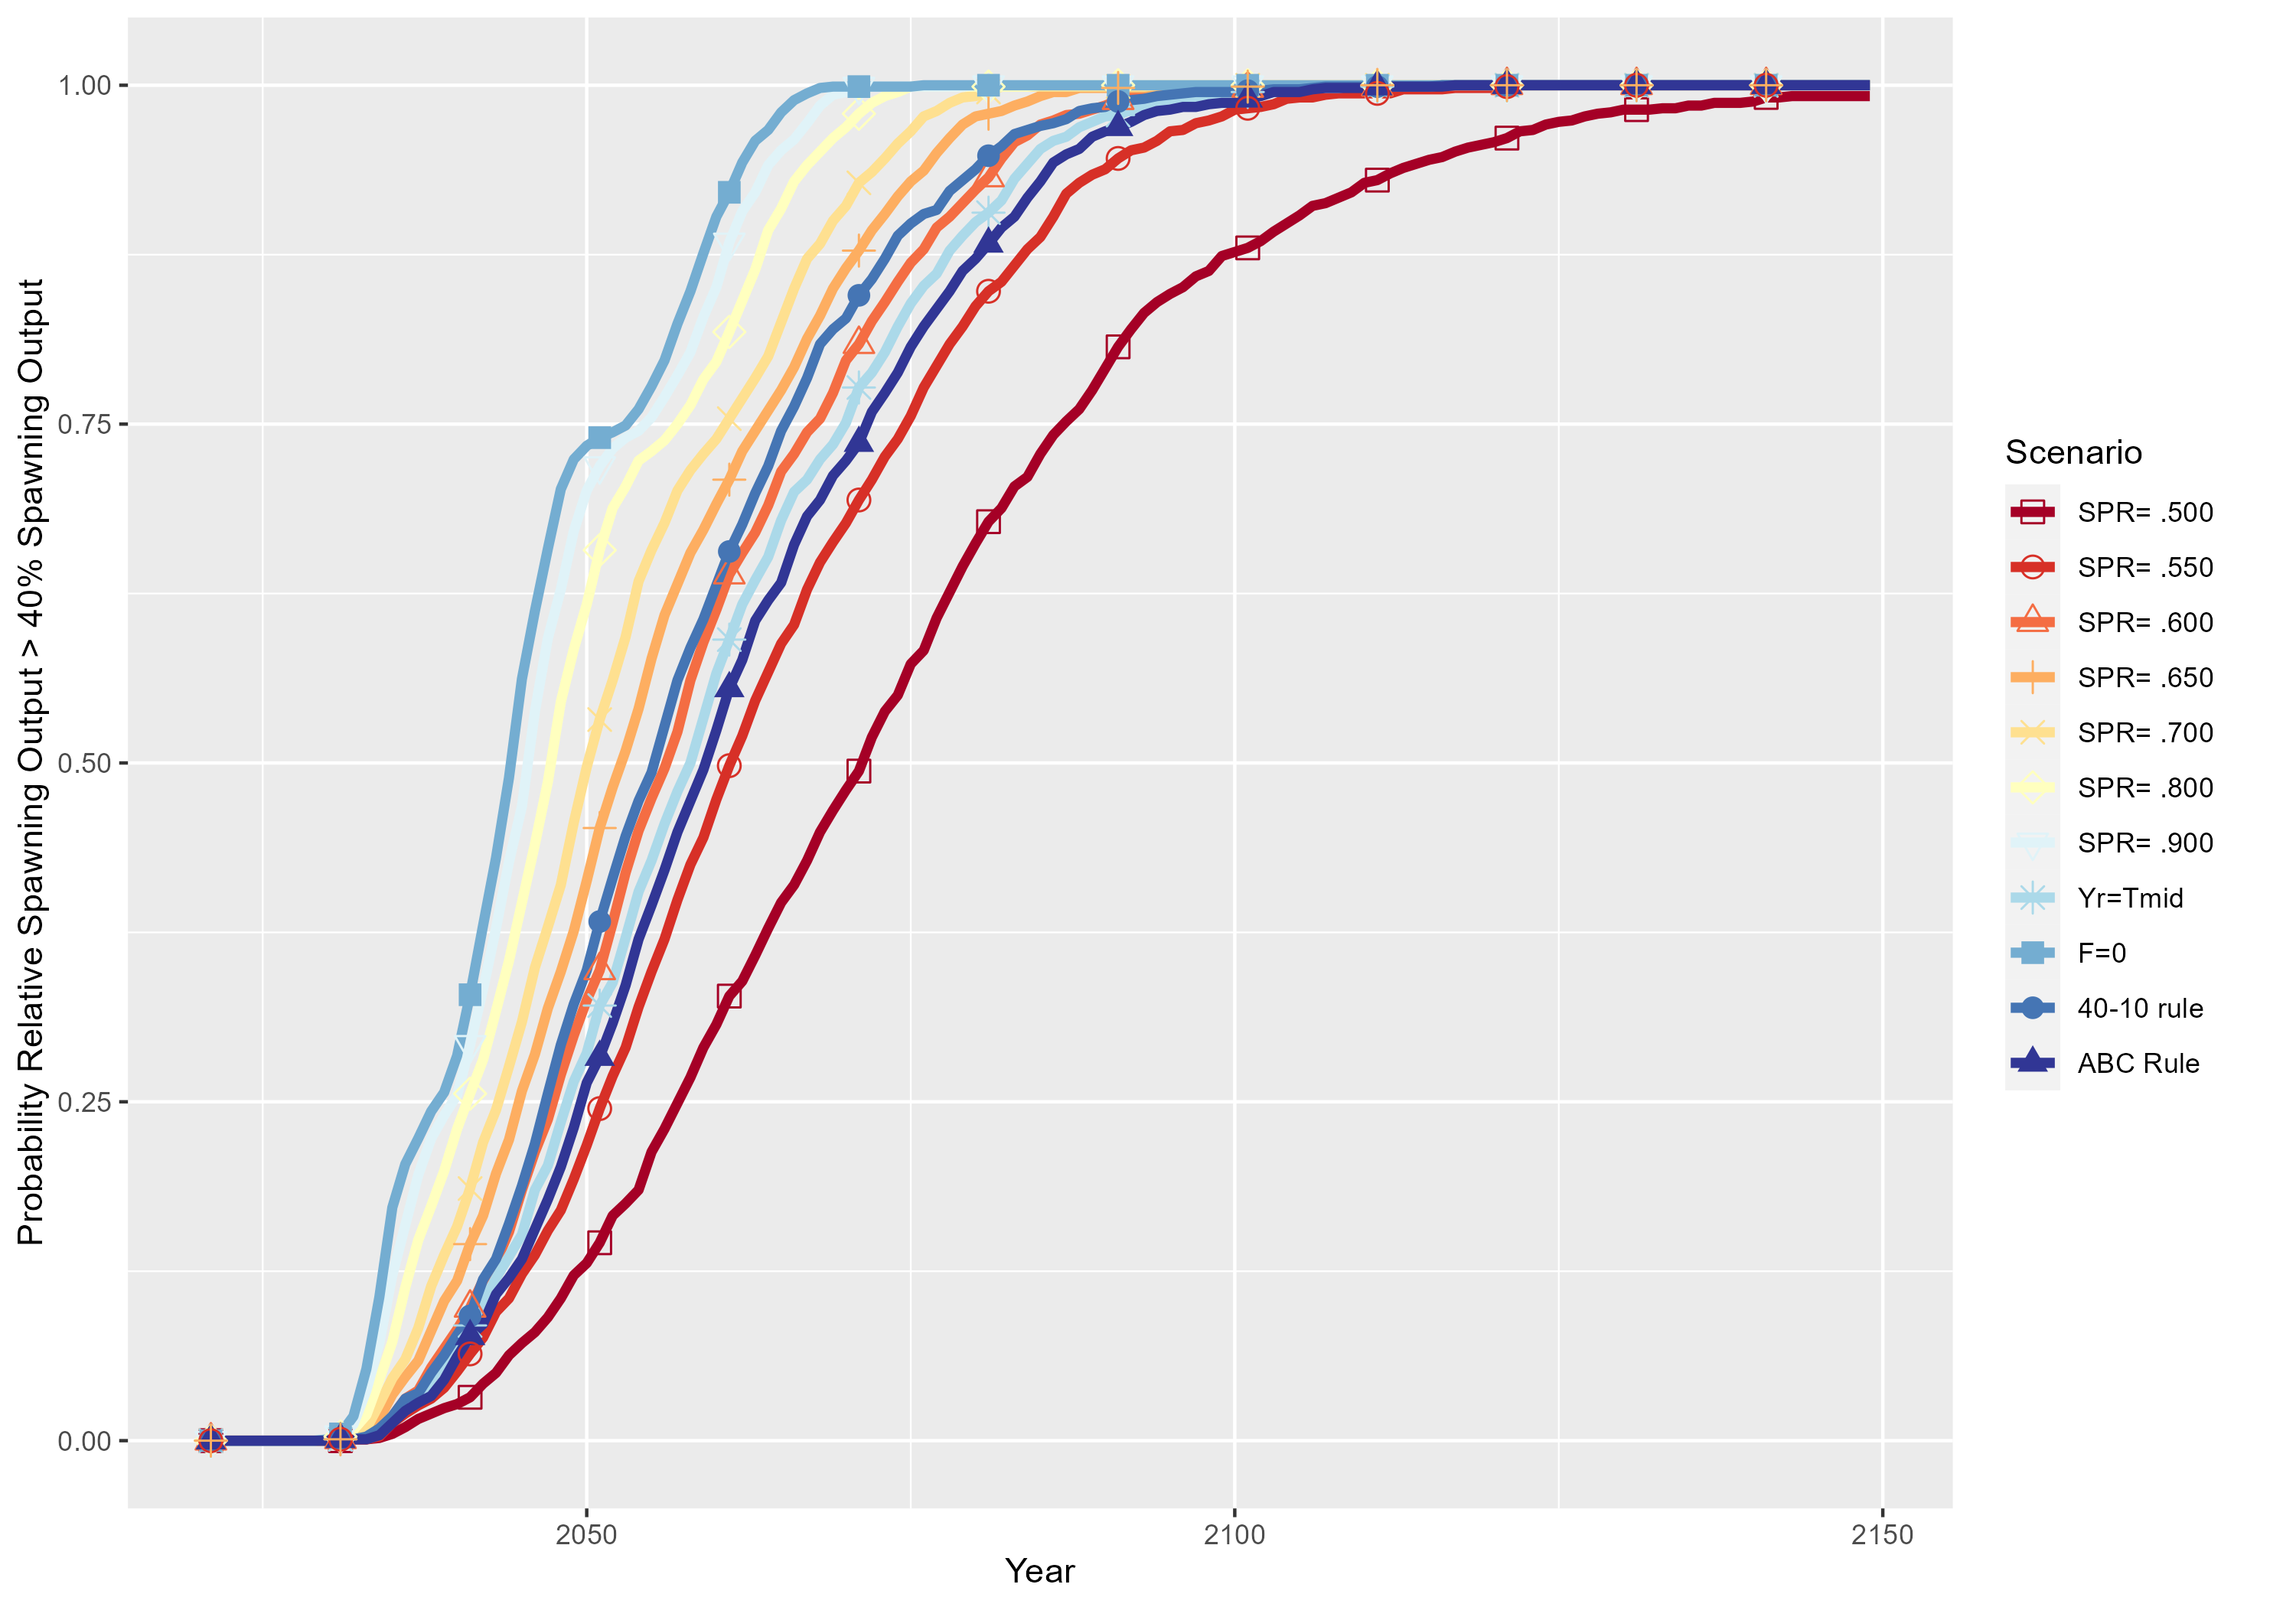
\includegraphics[alt=Line plot of probability of recovery by year after 2021 showing 11 lines that represent each rebuilding strategy.,width=1\textwidth,height=1\textheight]{C:/Users/Brian.Langseth/Desktop/ca/rebuilder/write_up_2023rebuild/figures/rebuilding_probability_forREPORT_relF.png}
}
\caption{Probability of rebuilding by year for the alternative rebuilding strategies.\label{fig:prob-fig}}
\end{figure}

\begin{figure}
{\centering
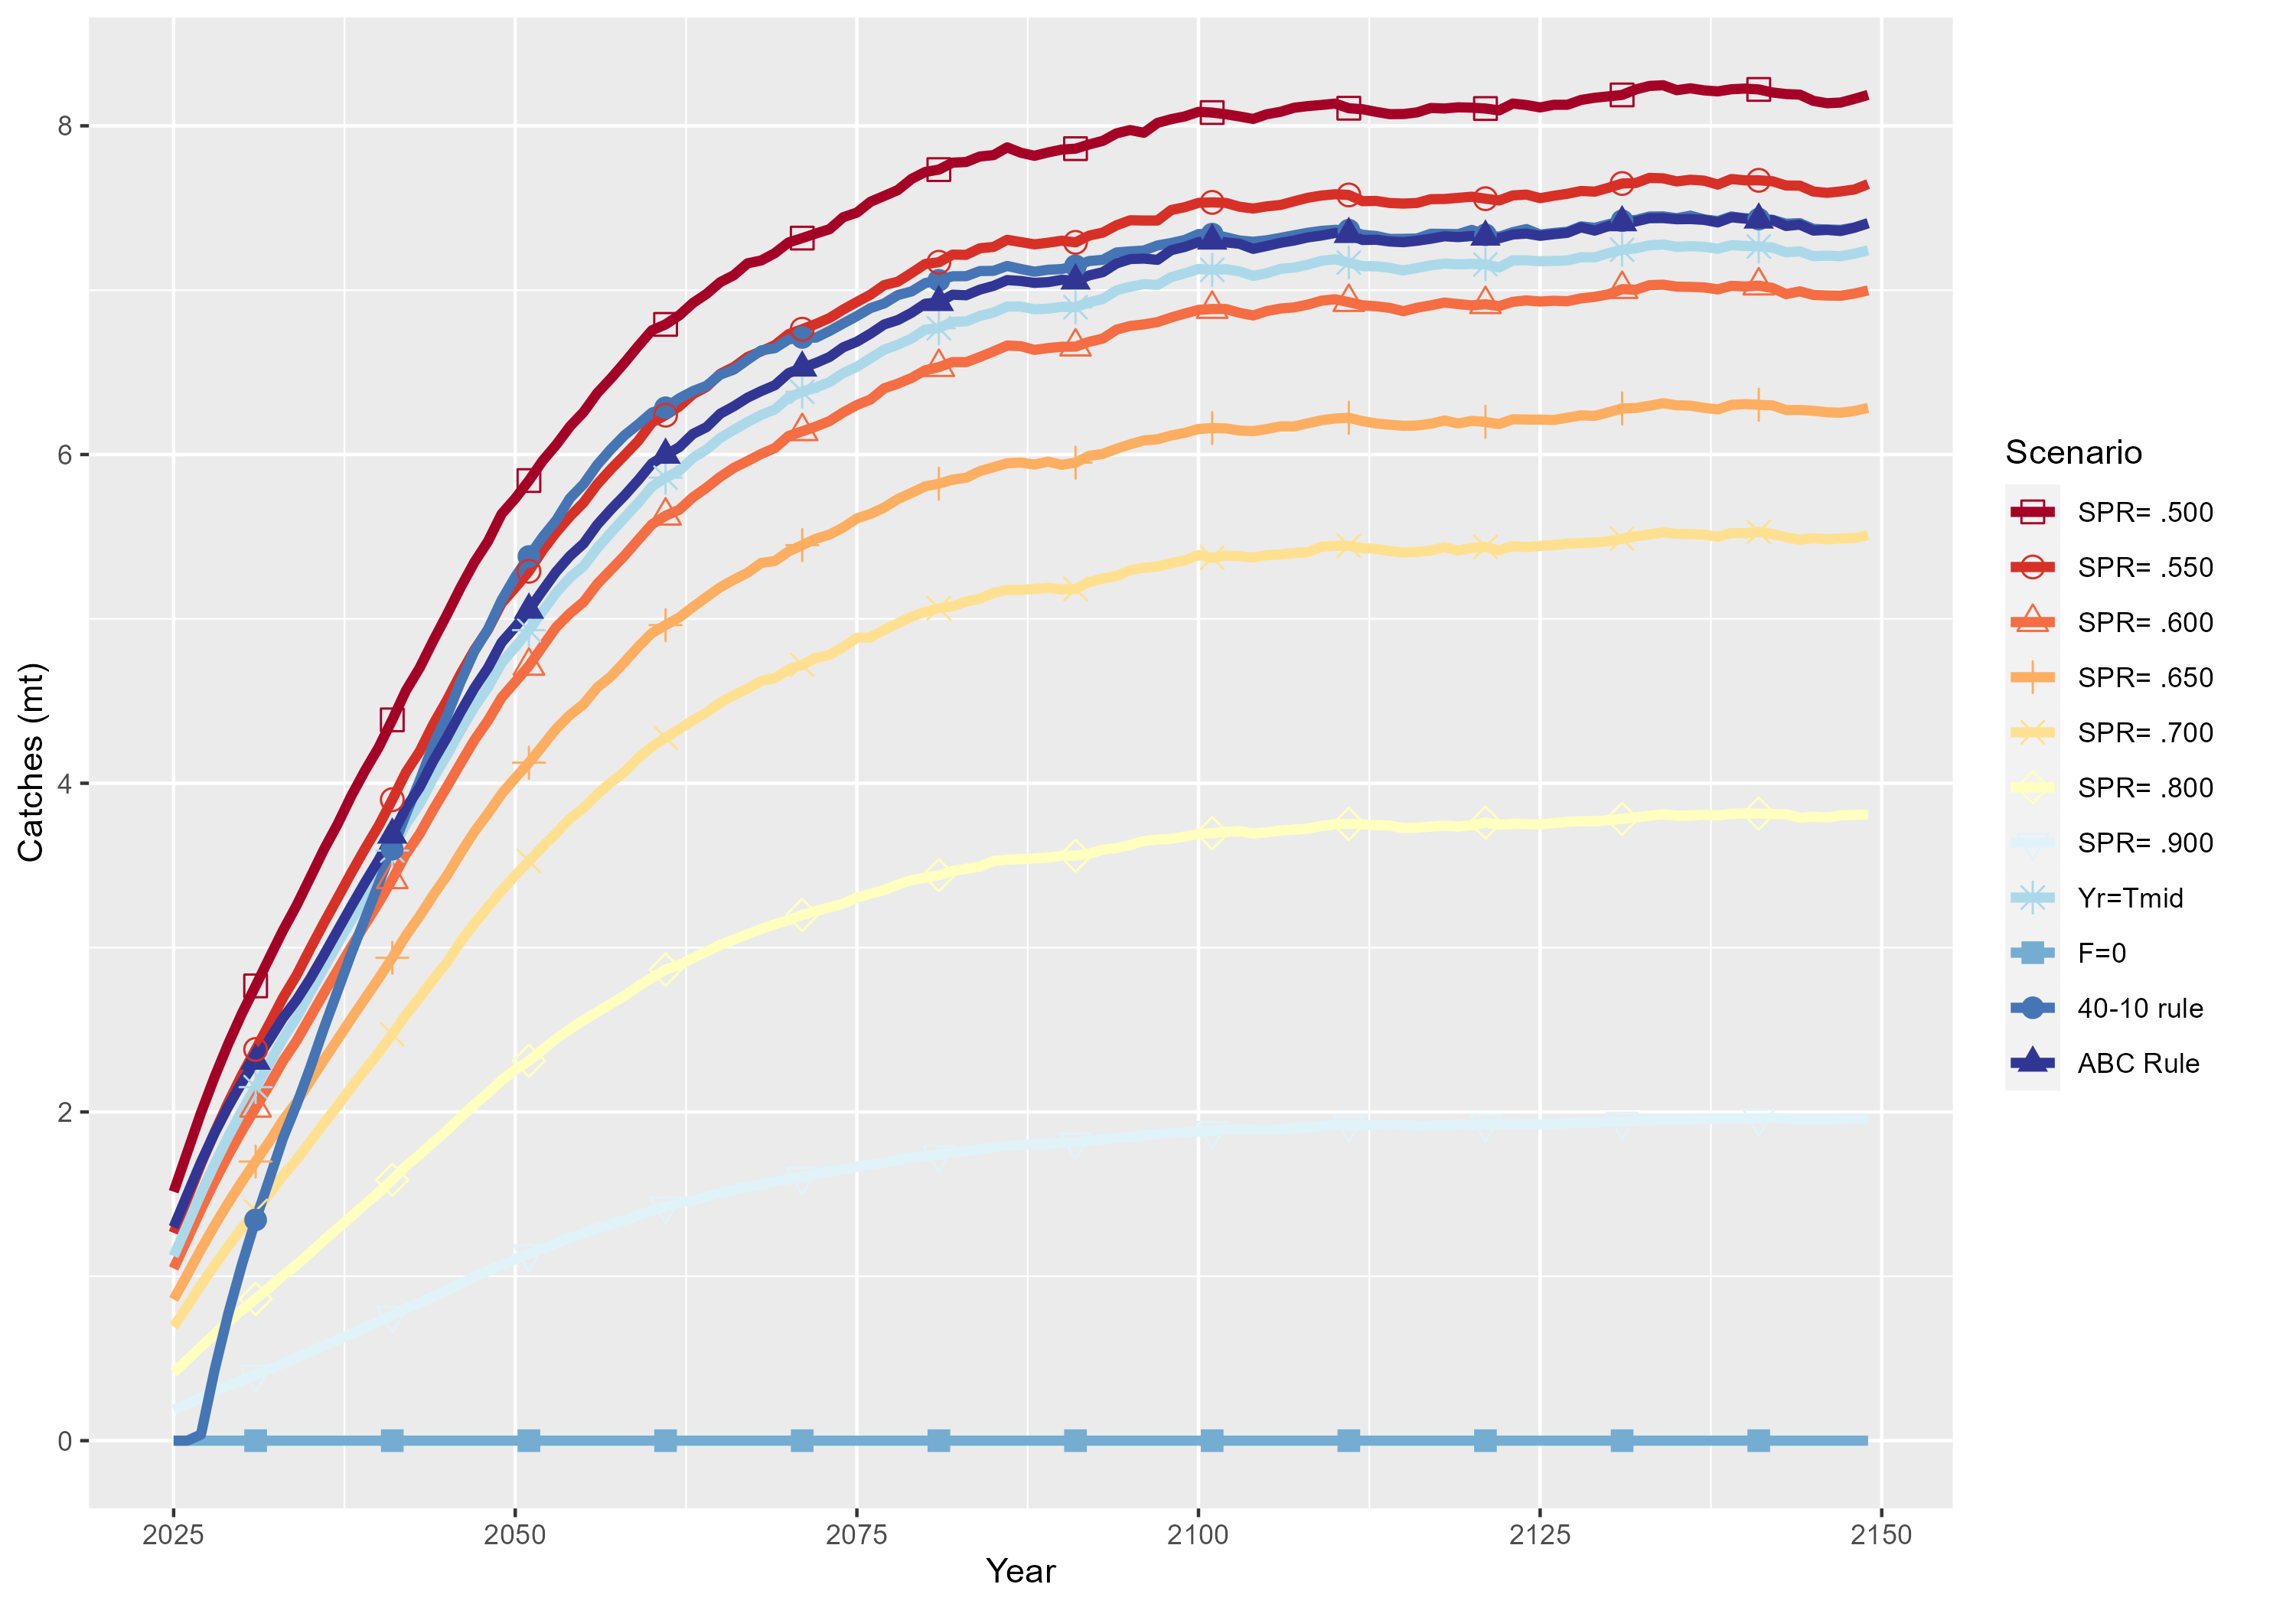
\includegraphics[alt=Line plot of catches by year after 2024 showing 11 lines that represent each rebuilding strategy.,width=1\textwidth,height=1\textheight]{C:/Users/Brian.Langseth/Desktop/ca/rebuilder/write_up_2023rebuild/figures/rebuilding_acl_forREPORT_relF.png}
}
\caption{Catches (mt) by year, starting in 2025, for the alternative rebuilding strategies.\label{fig:acl-fig}}
\end{figure}

\begin{figure}
{\centering
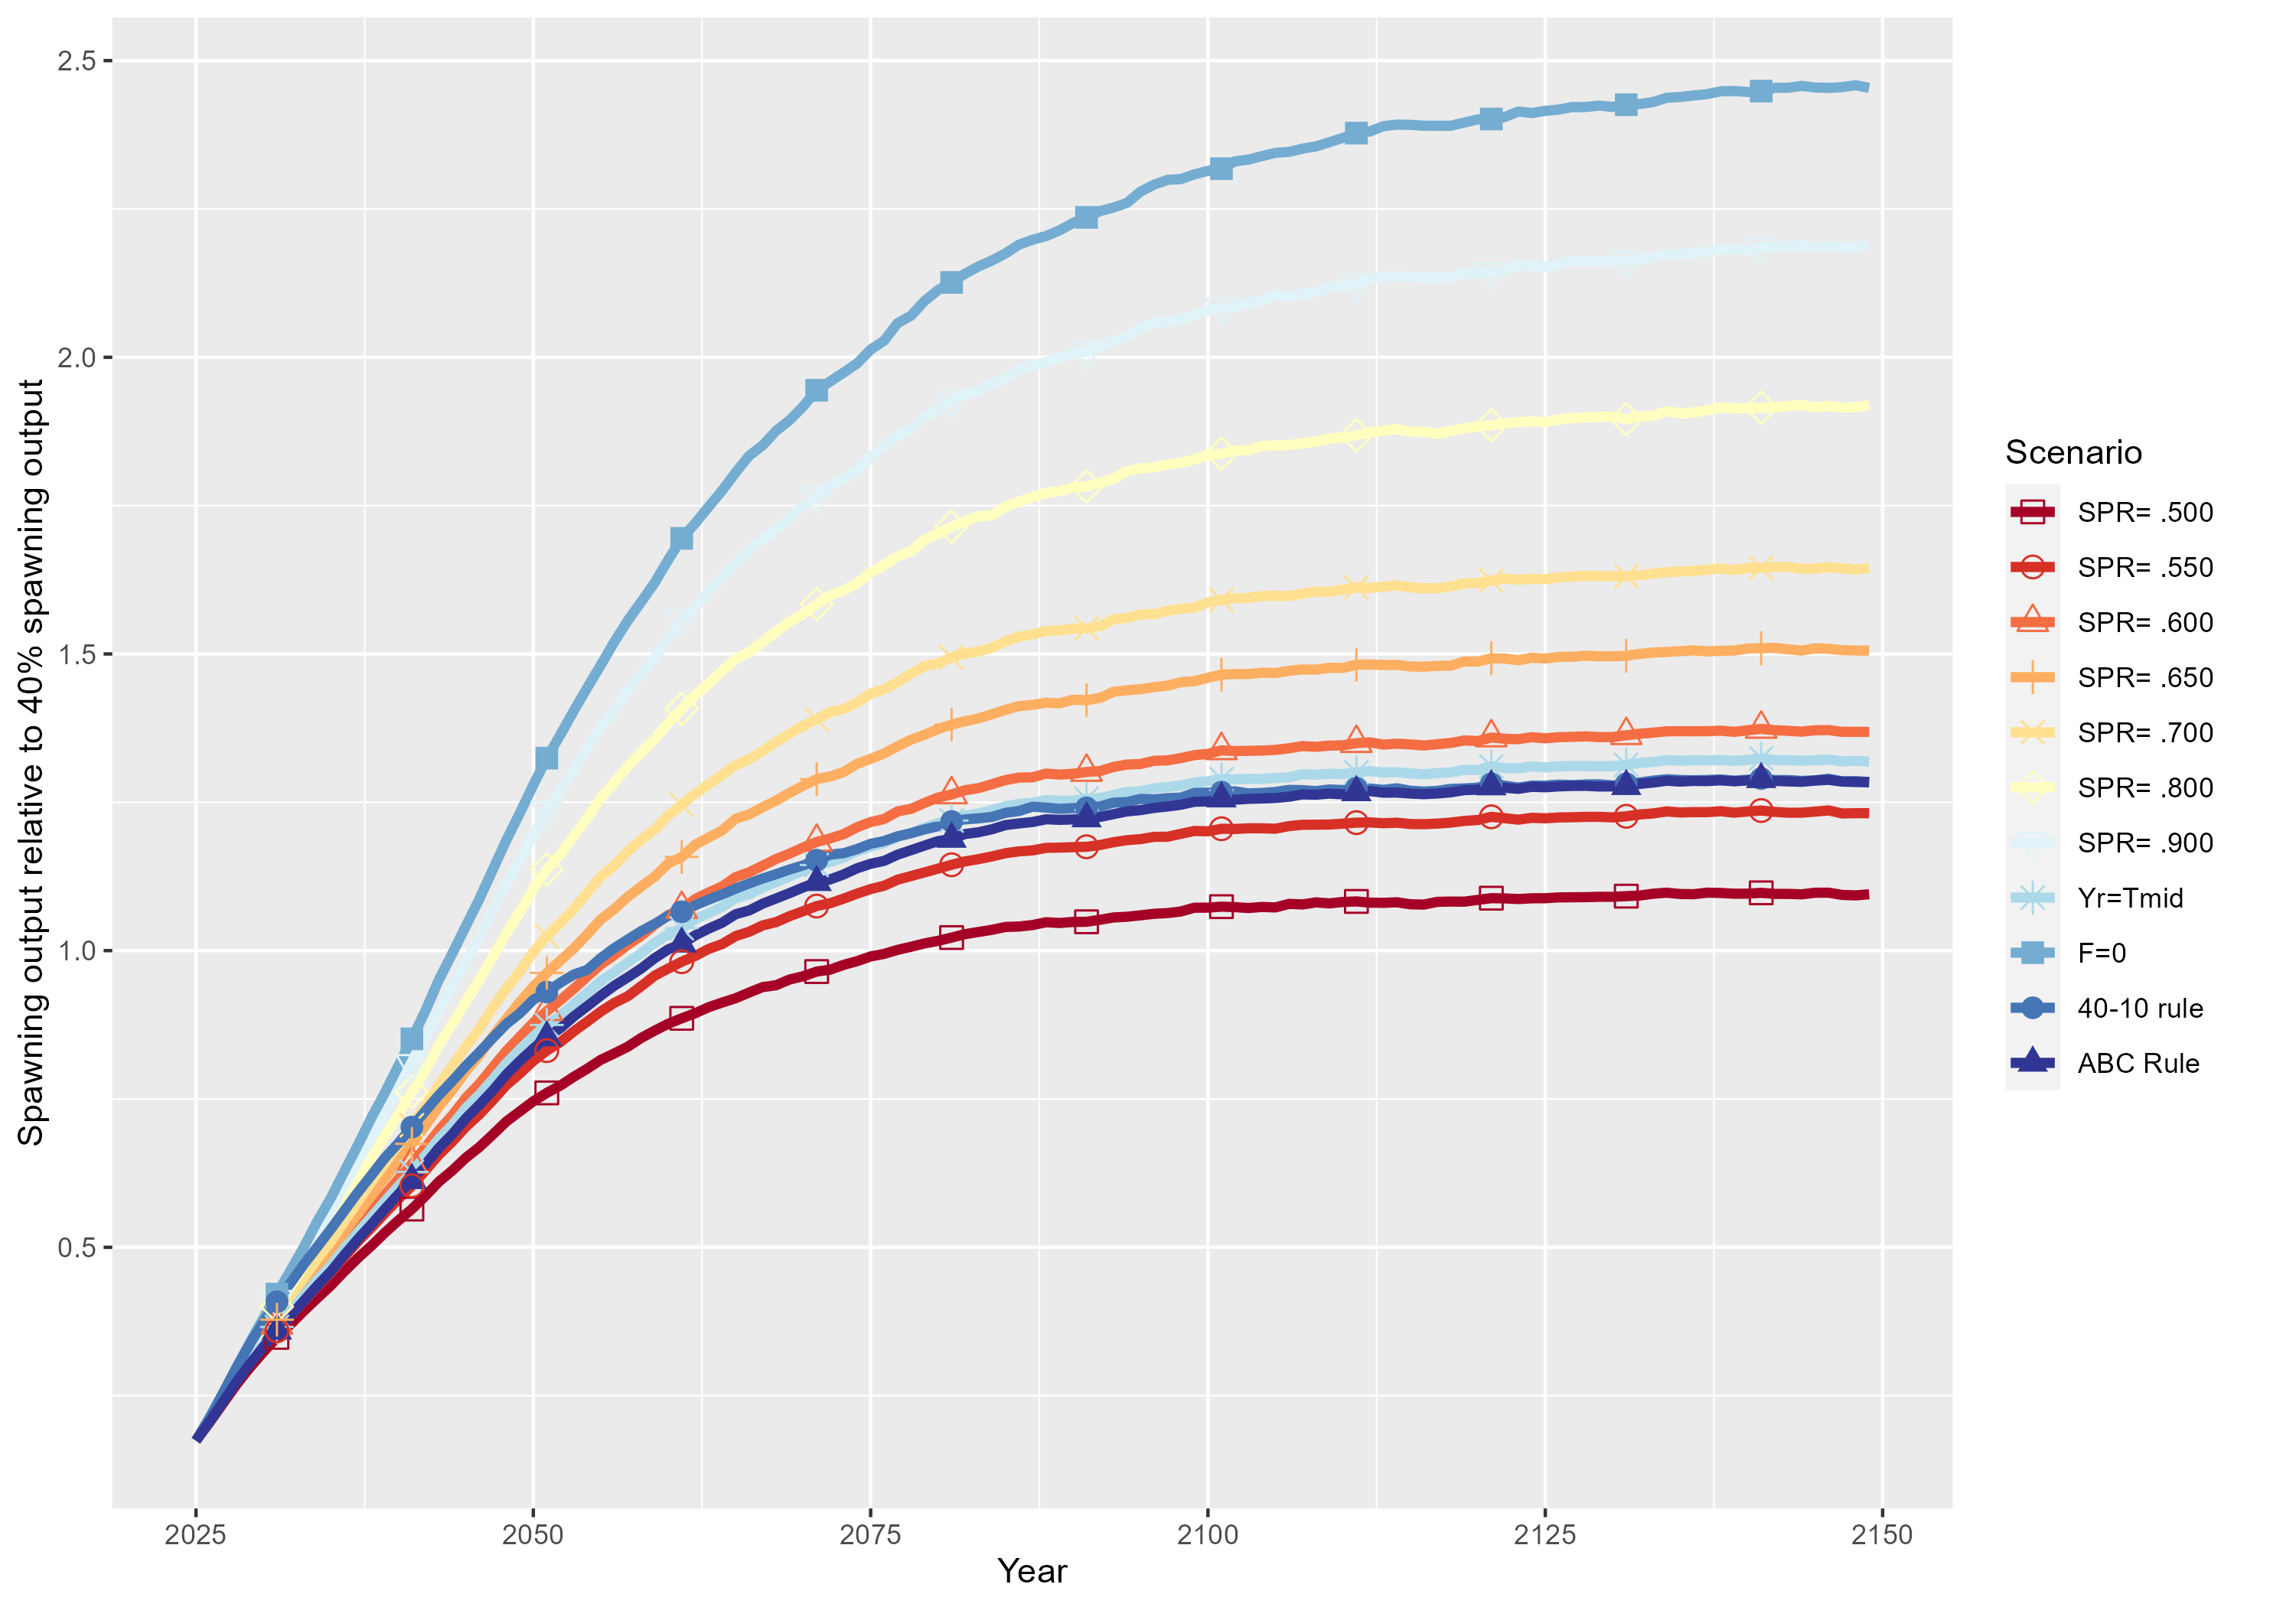
\includegraphics[alt=Line plot of relative spawning output by year after 2024 showing 11 lines that represent each rebuilding strategy.,width=1\textwidth,height=1\textheight]{C:/Users/Brian.Langseth/Desktop/ca/rebuilder/write_up_2023rebuild/figures/rebuilding_relative_sb_forREPORT_relF.png}
}
\caption{Spawning output relative to the management target of 40 percent of unfished spawning output by year, starting in 2025, for the alternative rebuilding strategies.\label{fig:rel-ssb-fig}}
\end{figure}

\begin{figure}
{\centering
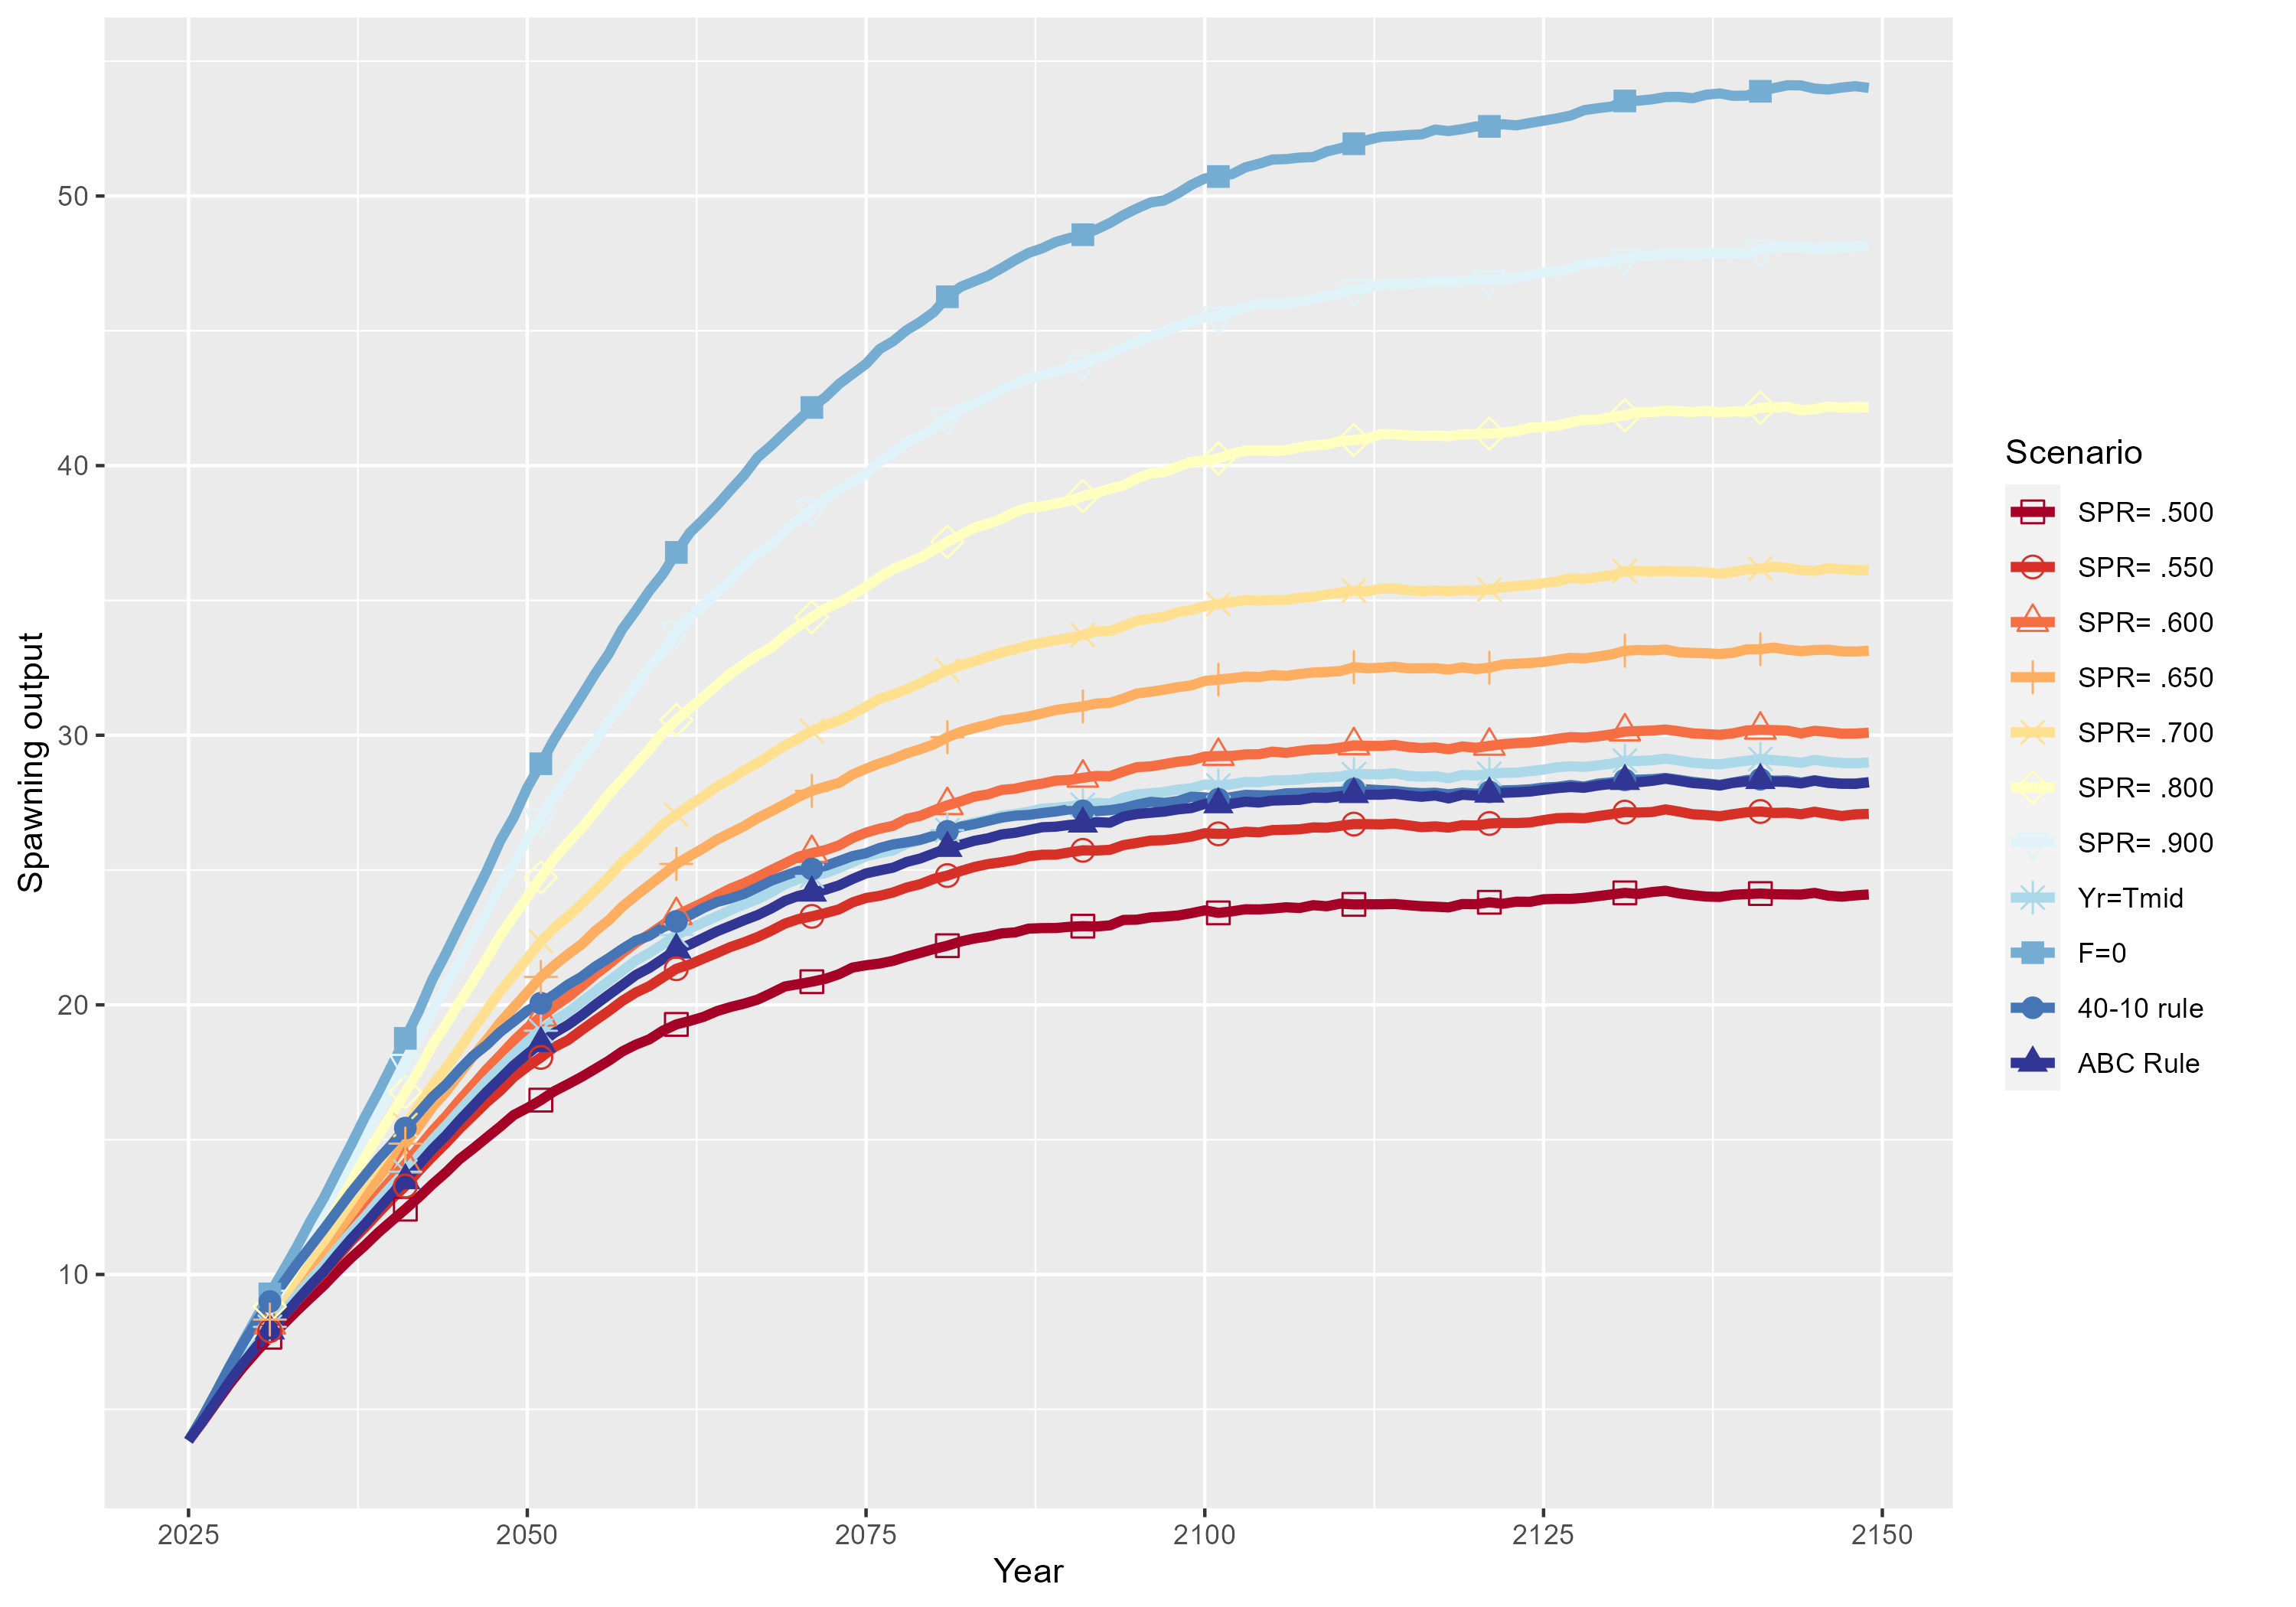
\includegraphics[alt=Line plot of spawning output by year after 2024 showing 13 lines that represent each rebuilding strategy.,width=1\textwidth,height=1\textheight]{C:/Users/Brian.Langseth/Desktop/ca/rebuilder/write_up_2023rebuild/figures/rebuilding_ssb_forREPORT_relF.png}
}
\caption{Spawning output by year, starting in 2025, for the alternative rebuilding strategies.\label{fig:ssb-fig}}
\end{figure}

\clearpage

\clearpage

\hypertarget{appendix}{%
\section{Appendix}\label{appendix}}

\hypertarget{append_a}{%
\subsection{Appendix A: Rebuilder data file}\label{append_a}}

The rebuild.dat file used for the base rebuilding analysis is provided below. Note that to achieve the SPR = 0.5 and SPR = 0.55 strategies, the option ``Constrain catches by the ABC'' had to be set to 2 (no).

\clearpage
\end{document}
